\documentclass[10pt,twocolumn]{article}
\usepackage[T1]{fontenc}
\usepackage[utf8]{inputenc}
\usepackage{times}
\usepackage[margin=0.75in]{geometry}
\usepackage{amsmath,amssymb}
\usepackage{graphicx}
\usepackage{booktabs}
\usepackage{multirow}
\usepackage[numbers,sort&compress]{natbib}
\usepackage[font=small,labelfont=bf]{caption}
\usepackage{microtype}
\usepackage{seqsplit}
\usepackage[hidelinks]{hyperref}
\usepackage{tikz}
\graphicspath{{figures/}}
% let floats share pages with text instead of taking a page each
\renewcommand{\topfraction}{0.9}\renewcommand{\bottomfraction}{0.8}\renewcommand{\textfraction}{0.08}\renewcommand{\floatpagefraction}{0.8}\renewcommand{\dbltopfraction}{0.9}\renewcommand{\dblfloatpagefraction}{0.8}\setcounter{topnumber}{3}\setcounter{bottomnumber}{2}\setcounter{totalnumber}{5}
\setlength{\columnsep}{0.25in}

\newcommand{\Sig}{\Sigma}
\newcommand{\Lz}{L_0}
\newcommand{\hash}[1]{\texttt{\seqsplit{#1}}}

\title{Decoder Spectra of Sparse Autoencoders against Covariance-Matched Sparse Nulls}
\author{Anonymous Authors}
\date{}

\begin{document}
\twocolumn[
\maketitle
\begin{abstract}
The eigenvalue spectrum of a sparse autoencoder's (SAE's) decoder directions falls as a power law whose slope has been read as a property of the model layer. On Gemma-2-2B the slope at a fixed layer rises by about 0.1 per doubling of the SAE's $L_0$. We compare real SAEs with SAEs trained on synthetic sparse data that has exactly the activations' covariance $\Sigma$ and the same reconstruction error. With equal power on every synthetic atom, real decoders are flatter in the bulk of the spectrum (ranks 31--1000) at all eight layers tested. Giving the atoms the real SAE's latent-power distribution produces 54--56\% of this gap at layer 13 and 28--32\% at layer 0, with a seed spread of about one point; across generator settings the share at layer 13 spans 43--78\%. These shares do not isolate feature power: the construction also aligns strong atoms with $\Sigma$, and its SAE concentrates latent power more than the real SAE. A remainder at least as large appears without a trained model, on random embeddings and after the first block of a randomly initialised Gemma-2-2B. Several predictions we fixed in advance failed. A low-powered test found no evidence that the slope predicts SAEBench quality beyond sparsity and reconstruction error.
\end{abstract}
\vspace{1em}
]

\section{Introduction}

\citet{li2025geometry} found that the decoder directions of Gemma Scope SAEs \citep{lieberum2024gemmascope} have a power-law covariance spectrum, steepest in the middle of the network, with a slope of $-0.47$ over ranks 11--150 at layer 12 of Gemma-2-2B. A replication on TopK SAEs found $-0.54$ to $-0.72$ \citep{peter2025progressive}. Statistics of this kind are used to argue about how a model organises its features. Before such an argument can rest on a spectrum, one needs to know how much of the spectrum an SAE would produce from data that shares only a few simple properties with the model's activations. This paper measures that for Gemma-2-2B.

Two properties are obvious candidates. The first is the SAE's operating point. Across 28 Gemma Scope SAEs at one layer of Gemma-2-2B the slope rises by 0.099 per doubling of the number of active latents $\Lz$, so two SAEs at the same layer can differ by more than Li et al.'s cross-layer effect. The second is the covariance $\Sig$ of the activations. An SAE trained on Gaussian samples with covariance $\Sig$ inherits part of $\Sig$'s spectrum, but it cannot code those samples sparsely (it leaves 52--60\% of the variance unexplained against 11--29\% on real data), so any comparison with it mixes data structure with operating regime. We therefore build a sparse synthetic source, a \emph{null}, whose covariance is exactly $\Sig$, whose atoms are random directions, and whose share of dense Gaussian variance is calibrated so that a TopK SAE \citep{gao2024scaling} trained on it has the real SAE's fraction of variance unexplained (FVU).

With equal power on every atom, this null's SAE has a bulk spectrum that falls about as steeply as $\Sig$'s. Real decoders are flatter at all eight Gemma-2-2B layers, at every $k$ from 8 to 128, and under every generator setting we tried. The bulk windows extend Li et al.'s fit over the next decade of ranks, which is where a power law that reflects feature organisation should still hold and where the difference from a null that shares only $\Sig$ is largest. Part of this difference is built into the null: an equal-power dictionary of $\Sig$-shaped atoms has a spectrum close to $\Sig$'s by construction, while real SAEs spread their power very unequally over latents.

We therefore built a second null whose atoms carry the real SAE's distribution of latent power. A power vector can be realised by a dictionary with covariance exactly $\Sig$ if and only if it is majorized by $\Sig$'s eigenvalues (the Schur--Horn theorem), so the covariance also pushes high-power atoms toward $\Sig$'s leading directions. At layer 13, in the reference generator setting, this power-matched null produces 54--56\% of the bulk gap, with a seed standard deviation of about one point over three SAE seeds, and one further dictionary draw agreed within 0.004. Across four generator settings at layer 13 the share is 43--78\%, and at layer 0 it is 28--32\%. The SAE trained on the power-matched null also ends up with more concentrated latent power than the real SAE, so the experiment shows what a null with real-like atom power produces; it does not isolate feature power as a cause of the gap. The remainder is produced by neither null. Nor does it need a trained model: on random token embeddings and after the first block of a randomly initialised Gemma-2-2B, the power-matched null leaves a remainder at least as large as on the trained model, by a rule fixed in advance (Section~\ref{sec:ladder}). We do not know what produces the remainder, and its presence on a trained model is therefore not by itself evidence about what the model has learned.

\textbf{Contributions.}
(1)~Evidence that the decoder slope is an operating-point statistic: a law in $\Lz$ at fixed layer, a layer profile that changes with $\Lz$, and a primary-window comparison with a null that spans $-0.19$ to $+0.13$ across generator settings. From these we derive a reporting protocol (Sections~\ref{sec:l0}, \ref{sec:equal} and \ref{sec:disc}).
(2)~A construction for a sparse null with covariance exactly $\Sig$ and a prescribed distribution of atom power, and a measurement of how much of that distribution an SAE trained on it recovers (Sections~\ref{sec:nulls} and \ref{sec:pmatch}, Appendix~\ref{app:pmatch}).
(3)~A partial decomposition of the bulk gap between real and null decoder spectra at matched covariance and reconstruction error, with its dependence on the generator (Section~\ref{sec:pmatch}), and a test showing that the part left unexplained is no smaller without a trained model (Section~\ref{sec:ladder}).
Appendix~\ref{app:prereg} lists every rule and prediction we fixed in advance and how it turned out.

\section{Related work}

\textbf{SAE decoder geometry.} \citet{li2025geometry} reported the power law, its mid-stack peak and cluster structure in Gemma Scope decoders, and left the origin of the power law open. \citet{peter2025progressive} found that larger TopK SAEs decay slightly less steeply; their larger SAEs also had larger $k$. \citet{borobia2026nearfloor} compare a geometric property of trained decoders with a matched i.i.d.\ control and count only the excess, which is the design we use for a different statistic.

\textbf{Nulls for SAEs.} SAEs trained on randomly initialised transformers score like trained ones on several interpretability metrics \citep{heap2025random}, and frozen random components match trained SAEs on probing and editing \citep{korznikov2026sanity}. Those nulls randomise the model; ours keep the activations' mean and covariance and randomise the features. \citet{engels2025darkmatter} show that much SAE error is linearly predictable from the input, which bears on how a null should generate the variance an SAE leaves uncoded.

\textbf{Data statistics and learned geometry.} Representation spectra are anisotropic \citep{ethayarajh2019contextual} and often follow power laws \citep{ghosh2022powerlaws}. In toy models, feature correlations shape the geometry of superposition \citep{prieto2026correlations}, and \citet{saraswatula2025whitening} argue that SAEs trained on unwhitened inputs are biased toward high-variance directions. \citet{michaud2025manifolds}, adapting \citet{brill2024scaling}, model how latents are allocated to features of different frequency. Feature splitting and absorption \citep{chanin2025absorption}, dense latents \citep{sun2025dense} and massive activations \citep{sun2024massive} are other candidate sources of decoder anisotropy; the first and the last have no measurable effect on the slope here (Appendix~\ref{app:fail}).

\textbf{Dictionary learning and frames.} SAEs are a form of sparse dictionary learning \citep{olshausen1996emergence,bricken2023monosemanticity}, and our nulls are the generative model that classical sparse coding assumes: independent sparse sources mixed by a fixed dictionary, here with a known covariance. Building a dictionary with prescribed atom norms and prescribed $A^\top A$ is the finite-frame problem of constructing a frame with given norms and frame operator. The Schur--Horn theorem \citep{horn1954doubly} gives the condition for existence, \citet{antezana2007schurhorn} state it for frames, and \citet{cahill2013constructing} give explicit constructions. We use an iterative construction that alternates the Gaussian optimal-transport map between two covariances \citep{olkin1982distance} with a rescaling of the atoms, because it starts from random directions and adds no structure beyond what the norms and $\Sig$ force. The Marchenko--Pastur law \citep{marchenko1967distribution} describes the simplest case of the finite-sample distortion of an empirical spectrum; we handle the corresponding bias in our slope ratio by simulation at a fixed number of rows (Appendix~\ref{app:live}). Latent power, as we measure it, weights the latent firing frequencies studied in earlier SAE work \citep{bricken2023monosemanticity} by the squared activation.

\section{Measuring a decoder spectrum}
\label{sec:setup}

An SAE with $n$ latents has unit-norm decoder rows $w_1,\dots,w_n \in \mathbb{R}^d$ ($d=2{,}304$ for Gemma-2-2B). We sort the eigenvalues $\lambda_1 \ge \lambda_2 \ge \dots$ of the rows' centred covariance and fit the least-squares slope of $\log_{10}\lambda_r$ on $\log_{10} r$ over a rank window $[a,b]$; a more negative slope means a more anisotropic cloud.

\textbf{Windows.} We fixed four windows before the experiments. Ranks 4--50 and 11--150 are the \emph{top windows}; the second is Li et al.'s window and our primary one. Ranks 31--450 and 101--1000 are the \emph{bulk windows}, which cover the next decade of ranks past the few dominant directions. The windows were not tuned, and they overlap, so agreement between neighbouring windows is weak corroboration. For other models each bound is scaled by $d/2{,}304$, which keeps every window at the same fraction of the dimension.

\textbf{Relative exponent.} $\Sig$ is the raw centred covariance of residual-stream activations. We report $\gamma = s_{\mathrm{dec}}/s_{\Sig}$, the decoder slope divided by $\Sig$'s slope in the same window. $\gamma=1$ means the decoder spectrum falls as steeply as $\Sig$'s and $\gamma<1$ that it falls less steeply. Against this covariance the decoder is flatter than $\Sig$ for both Gemma Scope SAEs we checked at each of the 26 layers of Gemma-2-2B, in every window, which seems to contradict Li et al.'s remark that activation spectra decay more slowly than feature spectra. Their protocol for the activations is not given, and if each dimension is standardised first their ordering does hold at middle layers (Appendix~\ref{app:li}), so the comparison depends on preprocessing.

\textbf{Fixed live count.} A finite cloud biases the slope. For our own TopK SAEs we use latents that fire on held-out tokens and score every SAE on 8,192 live rows drawn at random, averaged over four draws, so that all comparisons are at equal $n$. At this $n$ a Gaussian cloud whose covariance is exactly $\Sig$ reads $\gamma = 0.96$ in ranks 11--150 and in ranks 31--450, and 1.08 in ranks 101--1000 (Appendix~\ref{app:live}). Absolute values carry this bias; differences at equal $n$ largely cancel it. Gemma Scope SAEs are scored on all rows, as Li et al.\ did.

\textbf{SAEs.} We analyse 288 Gemma Scope residual-stream SAEs for Gemma-2-2B and 96 for Gemma-2-9b. Our own SAEs are TopK with an auxiliary loss for dead latents, width 16,384, trained for three passes over 9.5M Pile tokens and evaluated on 0.5M held-out tokens (Appendix~\ref{app:methods}). Real-data SAEs at $k=40$ have three seeds at each of eight layers of Gemma-2-2B (0, 3, 6, 9, 13, 17, 21, 24).

\section{Two sparse nulls}
\label{sec:nulls}

\begin{figure*}[t]
\centering
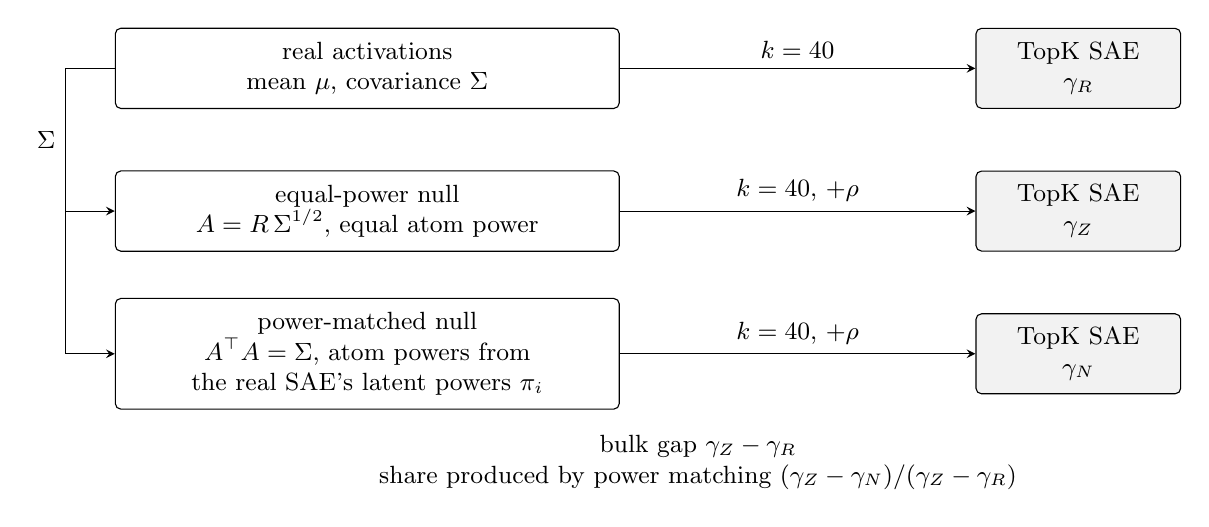
\begin{tikzpicture}[font=\small, >=stealth, x=2.1cm, y=1.45cm,
  box/.style={draw, rounded corners=2pt, align=center, inner sep=5pt, minimum width=6.4cm},
  sae/.style={draw, rounded corners=2pt, align=center, inner sep=5pt, minimum width=2.6cm, fill=black!5}]
\node[box] (act) at (0,0) {real activations\\ mean $\mu$, covariance $\Sig$};
\node[box] (ep) at (0,-1.25) {equal-power null\\ $A=R\,\Sig^{1/2}$, equal atom power};
\node[box] (pm) at (0,-2.5) {power-matched null\\ $A^\top A=\Sig$, atom powers from\\ the real SAE's latent powers $\pi_i$};
\node[sae] (R) at (4.3,0) {TopK SAE\\ $\gamma_R$};
\node[sae] (Z) at (4.3,-1.25) {TopK SAE\\ $\gamma_Z$};
\node[sae] (N) at (4.3,-2.5) {TopK SAE\\ $\gamma_N$};
\draw[->] (act) -- node[above]{$k=40$} (R);
\draw[->] (ep) -- node[above]{$k=40$, $+\rho$} (Z);
\draw[->] (pm) -- node[above]{$k=40$, $+\rho$} (N);
\draw[->] (act.west) -- ++(-0.3,0) |- node[pos=0.25, left]{$\Sig$} (ep.west);
\draw[->] (act.west) ++(-0.3,0) |- (pm.west);
\node[align=center] at (2.0,-3.45) {bulk gap $\gamma_Z-\gamma_R$\\ share produced by power matching $(\gamma_Z-\gamma_N)/(\gamma_Z-\gamma_R)$};
\end{tikzpicture}
\caption{The three-way comparison. Both nulls have covariance exactly $\Sig$ and random atom directions, and each adds a dense Gaussian share $\rho$ chosen so that its SAE matches the real SAE's FVU. The power-matched null takes one input from a real SAE, the distribution of its latent powers $\pi_i$. All $\gamma$ are measured at 8,192 live latents.}
\label{fig:schematic}
\end{figure*}

\textbf{Equal-power null.} Samples are
\[ x = \mu + \sqrt{1-\rho}\,(s-\mathbb{E}s)A + \sqrt{\rho}\,g, \qquad g \sim N(0,\Sig). \]
The $M=8{,}192$ rows of $A = R\,\Sig^{1/2}$ are the atoms, with $R$ a random $M\times d$ matrix with orthonormal columns, so $A^\top A = \Sig$ and every atom has the same expected power. The code $s$ has on average $L=16$ active entries per token, each one-signed half-normal with unit variance. The covariance of $x$ is $\Sig$ for every dense share $\rho$. At $\rho=0$ a $k=40$ SAE reconstructs these samples almost perfectly (FVU 0.013--0.016), far better than it reconstructs real activations. A calibration rule fixed before the runs therefore raised $\rho$ at each layer until the null SAE's FVU was within 0.03 of the real SAE's. All eight layers matched to within 0.02, with $\rho$ from 0.13 (layer 0) to 0.43 (layer 13). We call $(M,L)=(8192,16)$ with this dense share the reference setting. The calibrated share assumes that what a width-16,384 SAE leaves uncoded is dense Gaussian variance; Section~\ref{sec:equal} varies this.

\textbf{Power-matched null.} The second null changes $A$ (Figure~\ref{fig:schematic}). Write $P = AA^\top$. Its nonzero eigenvalues are those of $\Sig$ and its diagonal holds the atom powers $p_j = \|a_j\|^2$. By the Schur--Horn theorem a power vector is reachable with $A^\top A = \Sig$ exactly when it is majorized by $\Sig$'s eigenvalues: the $m$ largest powers sum to at most the $m$ largest eigenvalues, for every $m$. A dictionary with a few very strong atoms can therefore exist only if those atoms point along $\Sig$'s leading eigenvectors, so the covariance alone forces some alignment of power with direction. The construction allows this alignment and imposes no other structure. The target powers are the $M$ evenly spaced quantiles of the latent powers $\pi_i = \mathbb{E}[a_i^2]\,\|w_i\|^2$ of the seed-0 real SAE at the same layer, measured on 1M tokens and scaled to sum to $\mathrm{tr}\,\Sig$. Where the head of this distribution violates the bound it is capped just inside it; this moved 4.0\% of the power at layer 13 and none at layer 0. Directions start as in the equal-power null. The construction then alternates two steps: the least linear change that restores $A^\top A=\Sig$ (the Gaussian optimal-transport map from the current $A^\top A$ to $\Sig$), and a rescaling of each atom toward the target power of its current rank. Every dictionary we keep is the output of the first step, so its covariance is exact to a relative error of at most $1.5\times 10^{-12}$; on 1M samples drawn from the generator the error is 0.015--0.024. No real decoder direction enters; the only input from a real SAE is its list of powers (Appendix~\ref{app:pmatch}).

\textbf{What was fixed in advance.} The windows, the calibration rule and the decision rule and predictions of every run below were written down before that run. For the power-matched null, its later seeds, the run without a trained model (Section~\ref{sec:ladder}) and the quality analysis they are in dated notes; by our own record each note precedes the analyses it governs, and the job hashes stored in every result row of the power-matched runs and of the run without a trained model equal those in their notes. Appendix~\ref{app:prereg} gives the hashes, what they do and do not establish, every rule with its outcome, and the comparisons chosen after seeing data.

\section{Results}

\subsection{The slope depends on the operating point}
\label{sec:l0}

\begin{figure*}[t]
\centering
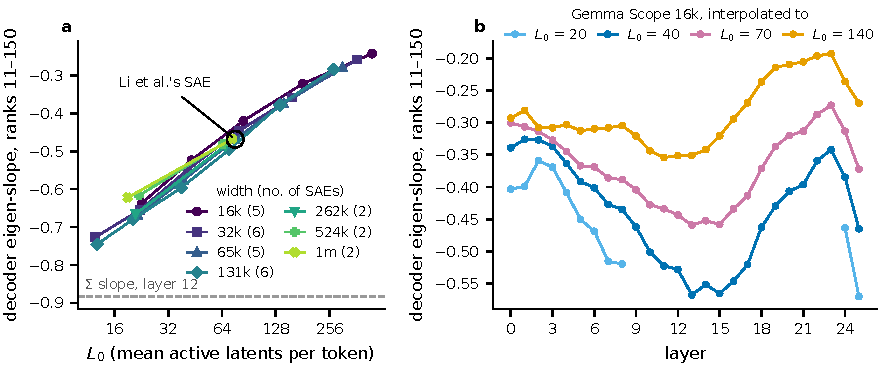
\includegraphics[width=\textwidth]{thesisA_fig1_setup.pdf}
\caption{At a fixed layer the decoder slope moves with sparsity. (a) Layer 12 of Gemma-2-2B, 28 Gemma Scope SAEs at seven widths, all decoder rows. The slope in ranks 11--150 rises by 0.099 per doubling of $\Lz$. \citeauthor{li2025geometry}'s SAE ($-0.468$, circled) lies on the line. The dashed line is $\Sig$'s slope (1M tokens). (b) Gemma Scope 16k decoders interpolated to fixed $\Lz$ across the 26 layers. The mid-stack minimum lies 0.23 below layer 0 at $\Lz=40$ and 0.06 at $\Lz=140$. Gaps mark layers whose SAEs do not bracket $\Lz=20$.}
\label{fig:l0}
\end{figure*}

If the slope were a property of the layer, SAEs at one layer should agree on it. They do not (Figure~\ref{fig:l0}a). Across the 28 Gemma Scope SAEs at layer 12, the slope in ranks 11--150 is linear in $\log_2\Lz$, rising by 0.099 per doubling ($R^2=0.984$) from $-0.73$ at $\Lz\approx 12$ to $-0.24$ at $\Lz\approx 444$. Width matters much less: SAEs of different width at matched $\Lz$ differ by 0.06--0.08. Li et al.'s SAE, at a measured $\Lz$ of 75.9, lies on the line. The larger SAEs of \citet{peter2025progressive} were also less sparse, which fits their finding that larger SAEs are flatter.

The layer profile changes with $\Lz$ too (Figure~\ref{fig:l0}b). With the 16k SAEs interpolated to a common $\Lz$, the mid-stack minimum is 0.23 below layer 0 at $\Lz=40$ and 0.06 below it at $\Lz=140$. $\Sig$ is also steepest mid-stack, and at $\Lz=40$ the decoder slope tracks $\Sig$'s slope across the 26 layers with Pearson $r=0.92$. Adjacent layers are far from independent, though. The effective sample size is 6.5, the 95\% interval for $r$ is $[0.50, 0.99]$, and at $\Lz=140$ the correlation falls to 0.37 (Appendix~\ref{app:corr}). We read this as consistent with $\Sig$ shaping the decoder and as weak evidence on its own.

The same descriptive facts hold, with less data, on two other models. Gemma Scope 16k SAEs for Gemma-2-9b show a slope that rises with $\Lz$ at the three layers with enough SAEs to fit it (0.089 per doubling in the primary window), a top window steeper mid-stack, and $\gamma<1$ for 92 SAEs with $\Lz\ge 20$, with one exception of 1.02. On GPT-2 small our own SAEs have $\gamma\le 0.82$ at all 12 layers, and $\gamma$ falls with $k$ at layer 6; there the top-window slope is steepest near the end of the stack (Appendices~\ref{app:gpt2} and~\ref{app:robust}).

The practical consequence is that a slope, or a layer profile of slopes, means little without the $\Lz$ at which it was measured. The comparisons below are therefore made between SAEs with the same $k$ and, against the nulls, the same FVU.

\subsection{Against an equal-power null}
\label{sec:equal}
\label{sec:primary}
\label{sec:bulk}

\begin{figure*}[t]
\centering
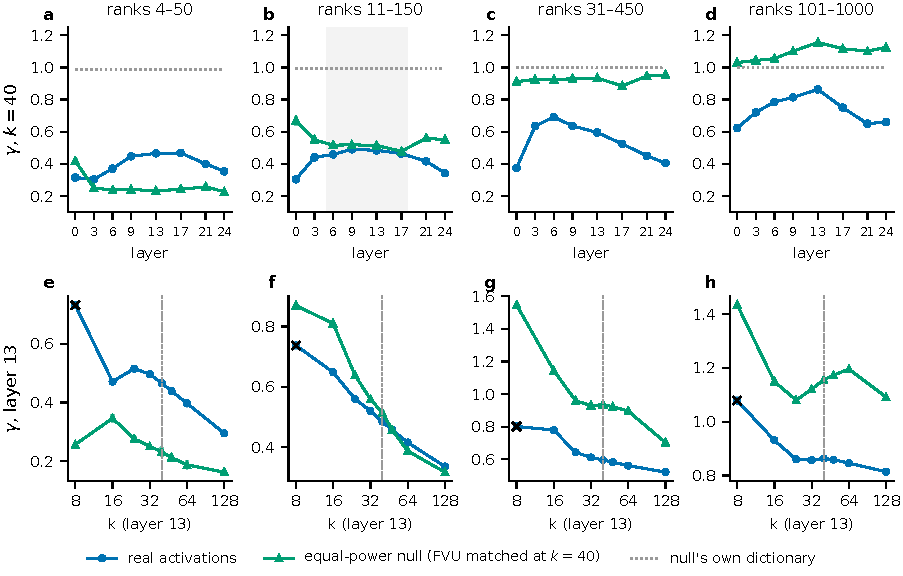
\includegraphics[width=\textwidth]{fig11_matched_null_r2.pdf}
\caption{$\gamma$ of real (blue, three seeds) and equal-power null (green, two seeds, reference setting) SAEs at 8,192 live latents; seed dots are mostly hidden by the markers. (a--d) Eight layers of Gemma-2-2B at $k=40$; dotted: the null's own dictionary. In ranks 11--150 the null is slightly steeper than real at layers 6--17 (shaded) and much steeper at the ends. In both bulk windows real is flatter at every layer. (e--h) Layer 13 over $k$, with $\rho$ fixed at its $k=40$ value (dashed line), so FVU is matched only there. $\times$: the real $k=8$ SAEs have fewer than 8,192 live latents and are scored on all of them.}
\label{fig:matched}
\end{figure*}

\textbf{The bulk.} In both bulk windows real decoders are flatter than the null's at all eight layers (Figure~\ref{fig:matched}c,d). The null SAEs have $\gamma$ of 0.88--0.95 in ranks 31--450 and 1.03--1.16 in ranks 101--1000, close to what an exact $\Sig$-shaped cloud reads at this $n$; real SAEs have 0.38--0.69 and 0.62--0.86. The gap is 0.23--0.55 and 0.27--0.46, and no 90\% interval from the seed spread comes closer to zero than 0.23. At layer 13 it holds at every $k$ from 8 to 128. It also holds under eight further generator settings at layers 13 and 0, in which we varied the number of atoms (4,096 or 32,768) or the number active per token (8 or 32), each recalibrated to the real FVU; at layer 13 we also replaced the dense share with a second sparse dictionary too large to code. Its size, however, depends on the generator: it ranges from 0.14 to 0.65 across these settings (Figure~\ref{fig:gen}, Appendix~\ref{app:robust}), and it is smallest with 32,768 atoms, a setting that matched the real FVU without any dense share. On GPT-2 small the same null at matched FVU leaves real flatter at all 12 layers in one bulk window, by 0.17--0.38; in the other window the gap is 0.11--0.50 and falls below 0.15 at the three layers where the null needed no dense share.

\textbf{The primary window.} Here the reference null is close to real at the middle layers and never on the other side of it. At layers 6--17 the null is steeper than real by 0.014 to 0.058 in $\gamma$; at layers 0, 3, 21 and 24 by 0.11 to 0.37. With three real and two null seeds the Welch intervals have 1.0 to 2.5 degrees of freedom, and they exclude zero at every layer except 17. The difference is one-sided, which is a small systematic offset, so we do not describe it as equivalence (Table~\ref{tab:matched} gives the intervals against a $\pm 0.06$ margin chosen after seeing the data). The closeness also belongs to the reference setting. At layer 13 the other generator settings put real minus null between $-0.19$ and $+0.13$, and the number of active atoms per token moves it most. In ranks 4--50 the sign of the difference depends on $\rho$ (Appendix~\ref{app:primary}).

So at middle layers the equal-power null at matched FVU reproduces the level of the primary-window $\gamma$ only within a generator-dependent band, from $-0.19$ to $+0.13$, while the real $\gamma$ itself varies by 0.03 across layers 6--17. The null does not pin this level down. The bulk gap is robust in sign, but part of it is built in: the null's own dictionary has $\gamma=0.99$--1.00 in every window, because all its atoms have equal power, and a TopK SAE that codes the null recovers something close to it. Any real dictionary with unequal latent power would differ from this null for that reason alone.

\subsection{Against a power-matched null}
\label{sec:pmatch}

\begin{figure*}[t]
\centering
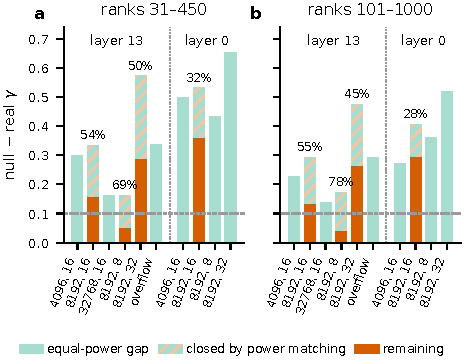
\includegraphics[width=0.8\textwidth]{fig14_generator_r2.pdf}
\caption{The bulk gap across generator settings, Gemma-2-2B, $k=40$, 8,192 live latents. Each bar is the equal-power null's $\gamma$ minus real's (three-seed mean) at one matched setting, labelled by $M$ (atoms) and $L$ (active per token); ``overflow'' replaces the dense share with an uncodable sparse dictionary. Where the power-matched null was run in its first run, the bar is split into the part it produces (hatched, share printed) and the part that remains (solid). Dashed line: 0.10, the margin within which the decision rule counts a window as closed. One SAE seed per null; the later power-matched run at 32,768 atoms and the three-seed values are in Table~\ref{tab:pmatch2} and Figure~\ref{fig:pmatch}.}
\label{fig:gen}
\end{figure*}

\begin{table*}[t]
\centering
\caption{The power-matched null against real and against the equal-power null at the same layer and $(M,L)$, $k=40$, first run: one SAE seed per null (real: three-seed mean); three-seed values are in Table~\ref{tab:pmatch2}. $\rho$ is the dense share, calibrated to the real FVU (targets 0.288 at layer 13 and 0.114 at layer 0); every setting matched at its first calibration run. ``\% closed'' is $(Z-N)/(Z-R)$ with $R$ real, $Z$ equal-power and $N$ power-matched. ``dict.\ 2'' is a second dictionary draw with new token streams. Verdict by the rule fixed in advance: \emph{explains} if both bulk windows end within 0.10 of real, \emph{does not} if either closes less than 30\%, \emph{partly} otherwise.}
\label{tab:pmatch}
\small
% generated by paper/figures/make_fig_null_r2.py from results/r2/runs_pmatch.jsonl, runs_sparse2.jsonl, runs_robust.jsonl and runs_real.jsonl
\begin{tabular}{l r r cc cr cr l}
\toprule
 & & & \multicolumn{2}{c}{$\gamma$: real / equal / matched} & \multicolumn{4}{c}{bulk: $\gamma$ real / equal / matched, \% closed} & \\
\cmidrule(lr){4-5}\cmidrule(lr){6-9}
layer, setting & $\rho$ & FVU & 4--50 & 11--150 & 31--450 & \% & 101--1000 & \% & verdict \\
\midrule
13, ref. & 0.43 & 0.282 & 0.47/0.24/0.24 & 0.48/0.51/0.42 & 0.60/0.93/0.75 & 54 & 0.86/1.16/0.99 & 55 & partly \\
13, dict. 2 & 0.43 & 0.281 & 0.47/0.24/0.23 & 0.48/0.51/0.42 & 0.60/0.93/0.75 & 55 & 0.86/1.16/0.99 & 57 & partly \\
13, $L$=8 & 0.43 & 0.272 & 0.47/0.16/0.19 & 0.48/0.36/0.35 & 0.60/0.76/0.65 & 69 & 0.86/1.03/0.90 & 78 & explains \\
13, $L$=32 & 0.42 & 0.293 & 0.47/0.32/0.24 & 0.48/0.68/0.50 & 0.60/1.17/0.88 & 50 & 0.86/1.34/1.13 & 45 & partly \\
0, ref. & 0.13 & 0.120 & 0.32/0.41/0.38 & 0.30/0.65/0.55 & 0.38/0.91/0.73 & 32 & 0.62/1.03/0.92 & 28 & does not \\
\bottomrule
\end{tabular}

\end{table*}

\begin{table*}[t]
\centering
\caption{Three SAE seeds of the power-matched null in the two reference settings and at layer 13 with 32,768 atoms ($L=16$, $k=40$). $R$: real, three-seed mean. $Z$: equal-power null at the same layer and $(M,L)$, mean of two seeds (reference) or three (32,768 atoms). $N$: power-matched null, mean $\pm$ sd over three seeds. ``\%'' is the closed fraction $(Z-N)/(Z-R)$ with its sd over the three $N$ seeds, $R$ and $Z$ held at their means. At 32,768 atoms the power-matched null needed $\rho=0.34$ to reach the real FVU while its equal-power comparator matched at $\rho=0$, so there $N$ and $Z$ differ in dense share as well as in atom power. Verdict by the rule of Table~\ref{tab:pmatch}.}
\label{tab:pmatch2}
\footnotesize
\setlength{\tabcolsep}{4pt}
% generated by experiments/r2_pmatch2_summary.py from results/r2_pm2/runs_pmatch2.jsonl and results/r2/runs_pmatch.jsonl, runs_sparse2.jsonl, runs_robust.jsonl, runs_real.jsonl
\begin{tabular}{l r rrrrr rrrrr l}
\toprule
 & & \multicolumn{5}{c}{ranks 31--450} & \multicolumn{5}{c}{ranks 101--1000} & \\
\cmidrule(lr){3-7}\cmidrule(lr){8-12}
layer, setting & $\rho$ & $R$ & $Z$ & $N$ & $N-R$ & \% & $R$ & $Z$ & $N$ & $N-R$ & \% & verdict \\
\midrule
13, ref. & 0.43 & 0.595 & 0.934 & 0.751$\pm$0.002 & 0.155 & 54$\pm$0.5 & 0.863 & 1.155 & 0.993$\pm$0.003 & 0.129 & 56$\pm$1.1 & partly \\
0, ref. & 0.13 & 0.375 & 0.912 & 0.738$\pm$0.004 & 0.363 & 32$\pm$0.7 & 0.623 & 1.030 & 0.916$\pm$0.001 & 0.292 & 28$\pm$0.1 & does not \\
13, $M$=32,768 & 0.34 & 0.595 & 0.750 & 0.650$\pm$0.007 & 0.054 & 65$\pm$4.2 & 0.863 & 0.996 & 0.940$\pm$0.004 & 0.076 & 43$\pm$2.9 & explains \\
\bottomrule
\end{tabular}

\end{table*}

We trained SAEs on the power-matched null of Section~\ref{sec:nulls} in six settings: the reference setting at layers 13 and 0, the same layer-13 setting with a new dictionary draw and new token streams, layer 13 with 8 and with 32 active atoms per token, and, in a later run, layer 13 with 32,768 atoms. Except at 32,768 atoms (below), everything other than the atom powers, and the alignment that the covariance forces on them, is as in the equal-power null at the same setting. The rule fixed before the first run classifies each bulk window as closed if the power-matched null ends within 0.10 of real, partial if it closes at least 30\% of the gap, and open otherwise. The two reference settings and the 32,768-atom setting have three SAE seeds each; there the power-matched null's bulk $\gamma$ has a seed standard deviation of 0.0005--0.004 in the reference settings and 0.004--0.007 at 32,768 atoms.

At layer 13 in the reference setting, matching power moves the null's bulk $\gamma$ from 0.93 and 1.16 to 0.75 and 0.99, against real's 0.60 and 0.86 (Figure~\ref{fig:gen}, Table~\ref{tab:pmatch}). That is 54\% and 55\% of the gap in the first run. Over three SAE seeds the null's $\gamma$ is $0.751\pm0.002$ and $0.993\pm0.003$, which closes 54\% and 56\% of the gap to the two-seed equal-power mean, with a seed standard deviation of 0.5 and 1.1 points (Table~\ref{tab:pmatch2}); the second dictionary draw lands within 0.004 of the first in both windows. At layer 0 the null moves from 0.91 and 1.03 to 0.74 and 0.92 (three seeds, sd 0.004 and 0.0005), against real's 0.38 and 0.62, closing 32\% and 28\% (sd 0.7 and 0.1 points). By the rule, layer 13 is partly explained and layer 0 is not, since one window closes less than 30\%, so the overall verdict is ``partly explains''. Both per-layer verdicts are the same with three seeds as with one. In the reference setting a gap of 0.13--0.16 at layer 13 and 0.29--0.36 at layer 0 is produced by neither null.

The top windows do not follow the bulk. In ranks 11--150 matching power moves the null from 0.03 steeper than real to 0.06 flatter (0.42 against 0.48), a shift of 0.09 against 0.16--0.18 in the bulk windows. In ranks 4--50 both nulls stay at 0.24, half of real's 0.47.

Layer 0 is the harder case for an account in terms of power. The real layer-0 SAE spreads its power much more evenly than the layer-13 SAE (its top 1\% of latents carry 11\% against 35\%), so the power-matched dictionary's own spectrum differs little from the equal-power one ($\gamma$ 0.86 against 1.00 in ranks 31--450), and yet layer 0 has the largest real-to-null gap.

\textbf{32,768 atoms.} Among the matched settings of the equal-power null, layer 13 with 32,768 atoms and 16 active per token has the smallest bulk gap, 0.155 and 0.133 (three seeds), and it reaches the real FVU with no dense share ($\rho=0$, FVU 0.309 against 0.288). We ran the power-matched null there to see whether, without a dense share, its SAE would lose the extra concentration of latent power described below. That design did not work as planned. With real-like atom power the data are much easier to reconstruct: at $\rho=0$ the SAE left FVU 0.083, so calibration raised $\rho$ to 0.34 (FVU 0.290), and the power-matched null at this setting has a dense share that its equal-power comparator does not. Over three seeds its bulk $\gamma$ is $0.650\pm0.007$ and $0.940\pm0.004$, 0.054 and 0.076 above real, so both windows are closed and by the rule power ``explains'' the gap at this setting. Closed is easy to reach here, because the equal-power gap is only 1.3--1.6 times the 0.10 margin, so the closed fraction is the number to read: 65\% and 43\% (seed sd 4.2 and 2.9 points), within the range of the other layer-13 settings. Since $N$ and $Z$ also differ in $\rho$, this fraction is not a clean measure of the effect of power. The dictionary is also milder than at 8,192 atoms. With four times as many atoms the target powers already satisfy the Schur--Horn bound, no power is moved by the cap, power and Rayleigh quotient correlate at only 0.08 (0.65 at 8,192 atoms), and the atoms' own $\gamma$ is 0.76 and 1.02 in the bulk windows, against 0.96 and 1.05 for equal-power atoms.

These results carry four qualifications. First, three of the six settings have three SAE seeds, and in them the closed share varies little: its seed standard deviation is 0.1--1.1 points in the reference settings and 3--4 points at 32,768 atoms, where the gap is smaller. This replaces the $\pm 5$-point band we had borrowed from the equal-power null's seed spread when each setting had one seed (Appendix~\ref{app:pmatch}). The settings with 8 and 32 active atoms and the second dictionary draw still have one seed each. Second, the share depends on the generator. With 8 active atoms per token both bulk windows end within 0.10 of real (69\% and 78\% closed), which by the rule ``explains'' the gap at that setting; with 32 the share is 50\% and 45\%. Part of this spread comes from the equal-power reference itself, which is 0.16--0.17 from real at $L=8$ and 0.47--0.57 from it at $L=32$. The 0.10 margin is about a third of the reference-setting gap at layer 13 (0.29--0.33) but about 60\% of the gap at $L=8$, so ``closed'' is much easier to reach in that setting. In absolute terms what remains at layer 13 is 0.04--0.05 at $L=8$, 0.13--0.16 at $L=16$, 0.26--0.29 at $L=32$ and 0.05--0.08 at 32,768 atoms. Third, the atoms of the power-matched null have the real power distribution, but the SAE trained on them does not. Its latents are more concentrated than the real SAE's: the top 1\% carry 53\% of the power against 35\% for real at layer 13, and 29\% against 11\% at layer 0 (three-seed means). The equal-power null's SAE is already concentrated (48\% and 27\%), because a few high-power latents code the dense share. At 32,768 atoms, where we had predicted the share would fall below 45\%, it stays at 51--53\% over three seeds at the matched $\rho=0.34$. The unmatched $\rho=0$ run has 22\%, so the dense share does drive the extra concentration; yet that run's bulk $\gamma$ (0.643 and 0.900) is within 0.001 and 0.035 of the matched seed-0 run's, although at a much lower FVU. What the comparison varies is therefore the power distribution of the SAE's input, together with the alignment of strong atoms with $\Sig$, and it does not isolate feature power. Fourth, the overall verdict is what we had predicted, but both per-layer predictions were the other way round, and we had expected the same verdict at all three values of $L$. For the later runs we predicted the verdict at 32,768 atoms and its closed fraction, the seed spread and both reference verdicts correctly, and the drop in latent-power concentration wrongly (Appendix~\ref{app:prereg}).

\subsection{Feature power in the real SAEs}
\label{sec:what}

A natural account of the remainder is that real SAEs concentrate power in a few latents aligned with $\Sig$'s leading directions, while the many weak latents are spread almost isotropically. We stated a rule for this before measuring power on retrained real SAEs: the structure is present at a layer if the power-weighted decoder cloud has bulk $\gamma$ within 0.25 of 1 and at least 0.15 above the unweighted cloud's, and if the latents outside the top 1\% by power have a median Rayleigh quotient $w^\top\Sig w/(\mathrm{tr}\,\Sig/d)$ below $10^{0.5}$. At layer 13 it is present. Weighting by power moves bulk $\gamma$ from 0.60 and 0.87 to 0.95 and 1.18, and the body's median quotient is 3.0 times a random direction's. At layer 0 it is absent: weighting moves $\gamma$ only from 0.37 and 0.62 to 0.51 and 0.68. Both null SAEs fail the rule. The rule asked for four real layers before giving a verdict across layers, and we retrained real SAEs at the two layers the power-matched null needed, so it gives none. This head-and-body picture fits layer 13, where power matching also produces the larger share, and does not fit layer 0. Analyses of earlier Gemma Scope SAEs and of the decoder covariance in $\Sig$'s eigenbasis are in Appendix~\ref{app:local}.

\subsection{Without a trained model}
\label{sec:ladder}

\begin{table*}[t]
\centering
\caption{The real / equal-power / power-matched comparison with and without a trained model, $k=40$, $\gamma$ at 8,192 live latents. Each dataset has its own $\Sig$. FVU: mean of the three real SAEs; $\rho$: the dense share at which both nulls matched it (within 0.03). $R$: real, three seeds; $Z$: equal-power null, two seeds; $N$: power-matched null, one seed; $G=Z-R$; Rem $=N-R$. embT: trained Gemma-2-2B input embeddings; embR: random embedding matrix; randL0, randL13: blocks 0 and 13 of a randomly initialised Gemma-2-2B. Gemma rows are the existing results ($Z$ two seeds, $N$ the first run's seed 0, as the rule specifies). Verdict by the rule fixed in advance, against the Gemma row above it; in brackets the ratio of the random dataset's remainder to the trained one in the two bulk windows (``persists'' needs at least 0.70 in both). $^\dagger$The rule's verdict; we read randL13 as uninformative in practice (see text).}
\label{tab:ladder}
\footnotesize
\setlength{\tabcolsep}{3pt}
% generated by paper/figures/make_fig_ladder.py from results/r2/ladder_summary.json
\begin{tabular}{l rr rrrrr rrrrr l}
\toprule
 & & & \multicolumn{5}{c}{ranks 31--450} & \multicolumn{5}{c}{ranks 101--1000} & \\
\cmidrule(lr){4-8}\cmidrule(lr){9-13}
dataset & FVU & $\rho$ & $R$ & $Z$ & $N$ & $G$ & Rem & $R$ & $Z$ & $N$ & $G$ & Rem & verdict (Rem ratio) \\
\midrule
embT (Gemma emb.) & 0.044 & 0.05 & 0.313 & 0.869 & 0.680 & 0.556 & 0.367 & 0.574 & 0.953 & 0.837 & 0.379 & 0.262 & reference \\
embR (random emb.) & 0.085 & 0.12 & 0.192 & 0.863 & 0.699 & 0.671 & 0.507 & 0.456 & 0.988 & 0.859 & 0.532 & 0.403 & persists (1.38, 1.53) \\ \addlinespace
Gemma, block 0 & 0.114 & 0.13 & 0.375 & 0.912 & 0.734 & 0.537 & 0.359 & 0.623 & 1.030 & 0.915 & 0.407 & 0.292 & reference \\
randL0 & 0.295 & 0.40 & 0.402 & 1.023 & 0.951 & 0.621 & 0.549 & 0.727 & 1.177 & 1.113 & 0.451 & 0.386 & persists (1.53, 1.32) \\ \addlinespace
Gemma, block 13 & 0.288 & 0.43 & 0.595 & 0.934 & 0.751 & 0.339 & 0.155 & 0.863 & 1.155 & 0.994 & 0.292 & 0.130 & reference \\
randL13 & 0.601 & 0.86 & 0.875 & 1.449 & 1.429 & 0.575 & 0.554 & 1.161 & 2.649 & 2.256 & 1.489 & 1.095 & persists$^\dagger$ (3.57, 8.40) \\
\bottomrule
\end{tabular}

\end{table*}

\begin{figure*}[t]
\centering
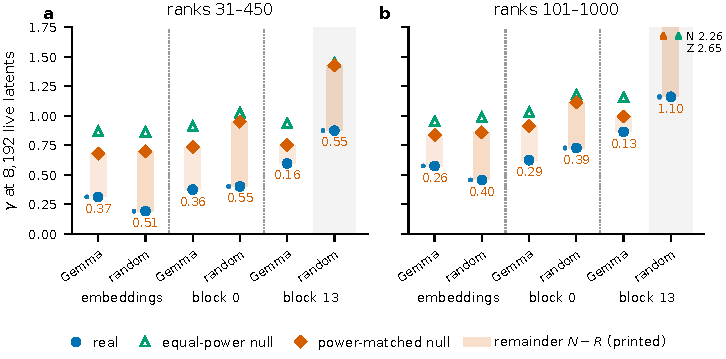
\includegraphics[width=0.85\textwidth]{fig15_ladder.pdf}
\caption{The remainder with and without a trained model. For each pair: the trained Gemma-2-2B dataset and the same input or layer without trained weights (random embedding matrix; randomly initialised model). Real (blue; small dots: seeds), equal-power null (green) and power-matched null (orange); the shaded bar and the printed number are the remainder $N-R$. At block 13 of the random model (grey) the equal-power null sits just behind the power-matched one in ranks 31--450, and both are off the axis in ranks 101--1000 (values printed); there the nulls are 86\% dense Gaussian and their bulk spectra are not straight (see text).}
\label{fig:ladder}
\end{figure*}

Both nulls take $\Sig$ as given and remove what SAE training on real features adds. They do not remove the model's own training, which shapes $\Sig$ and everything else about the activations. A second run, which we call the ladder, asks whether the remainder needs a trained model at all. It repeats the three-way comparison on four datasets of 10M Pile tokens each: the trained Gemma-2-2B input embeddings with no transformer block (embT); the same with an i.i.d.\ Gaussian embedding matrix of equal overall RMS (embR); and the residual stream after blocks 0 and 13 of a Gemma-2-2B with every weight at its default random initialisation (randL0, randL13). Each dataset gets its own $\Sig$, three real SAEs, an equal-power null with two SAE seeds and a power-matched null built from its own seed-0 real SAE's latent powers, both calibrated to the real FVU by the rule used before. A rule fixed before the run compares each random dataset with its trained counterpart (embR with embT, randL0 and randL13 with trained layers 0 and 13): the remainder \emph{persists} if it is at least 0.70 of the trained remainder in both bulk windows, is \emph{absent} if it is below 0.10 in both, and is \emph{partial} otherwise; the comparison is uninformative if the trained remainder is below 0.10 or a null is missing or unmatched.

Without a trained model the remainder is not smaller (Table~\ref{tab:ladder}, Figure~\ref{fig:ladder}). With a random embedding matrix it is 0.51 and 0.40 in the two bulk windows, against 0.37 and 0.26 for the trained embeddings. After block 0 of the random model it is 0.55 and 0.39, against 0.36 and 0.29 for trained layer 0. All eight ladder nulls matched the real FVU, no SAE entering $R$, $Z$ or $N$ was short of 8,192 live latents, and by the rule both comparisons \emph{persist}, with ratios of 1.32--1.53 that are far from the 0.70 line (randL13 also returns ``persists''; see below). Both random datasets also keep a large equal-power gap (0.45--0.67). The power-matched null closes a smaller share of that gap on the random datasets than on the trained ones (24\% on embR, 12--14\% on randL0, against 31--34\% on embT and 28--33\% on trained layer 0). The supported statement is therefore that a trained model is not needed to produce a remainder of this size under this null. It does not follow that the remainder has the same cause with and without training. The datasets differ in $\Sig$, in real FVU (0.044--0.295 across embT, embR and the two block-0 datasets) and in the dense share their nulls need, and the rule compares sizes, not mechanisms. One case is still informative about what the remainder can be. In embR every token is a single random Gaussian vector, so the data are a one-sparse mixture of random directions whose power is set by token frequency, and there are no learned directions for the real SAE to arrange. A remainder of 0.51 and 0.40 there must come from how the null's source differs from such data (16 active atoms per token instead of one, a dense share, the alignment its covariance forces) or from how a TopK SAE treats each source.

These results carry three qualifications, with details in Appendix~\ref{app:ladder}. First, randL13 is degenerate in practice, although no stop rule fires and the rule returns ``persists''. Its $\Sig$ is not the problem: its top eigenvalue carries 4.0\% of the variance and its participation ratio is 234 (trained layer 13: 6.3\% and 111), and $\Sig$'s bulk fits have $R^2\ge 0.998$ with slopes of $-0.72$ and $-0.75$, so $\gamma$'s denominator is stable. The problem is that a $k=40$ SAE leaves 60\% of its variance unexplained, so both nulls need a dense share of 0.86 and are mostly Gaussian. Their decoder spectra then bend inside the bulk windows: in ranks 31--450 the equal-power null's $\gamma$ is 0.81 over the lower half of the window and 1.94 over the upper half, and the log-log fits reach $R^2$ of only 0.93. $Z$ also depends on the dense share more than on anything else: it is 1.00 and 1.11 at the first calibration point ($\rho=0.30$) and 1.45 and 2.65 at the accepted $\rho=0.86$. The remainder at randL13 (0.55 and 1.10) therefore mostly measures the null's dense share, and we treat this comparison as uninformative in practice. Second, the embedding datasets contain one vector per token type. The FVU match is not trivial there (real FVU 0.044 and 0.085, $\rho$ 0.05 and 0.12), and real SAEs with $k=4$ and $k=16$ give bulk $\gamma$ within 0.06 of $k=40$, but these data are a finite, frequency-weighted set of points and far from the residual stream; their nulls' SAEs also leave more latents dead (9,079--12,770 of 16,384 live, all above 8,192). Third, the power-matched nulls have one SAE seed and the comparison rests on one random initialisation; on the trained model, in the reference settings, the power-matched null's seed standard deviation was at most 0.004 in the bulk windows, and replacing the trained $N$ by its three-seed mean changes the ratios by at most 0.07. As on the trained model, the SAE trained on each power-matched null concentrates its latent power more than the real SAE (top 1\% of latents: 0.39--0.52 against 0.11--0.24), although each dictionary's top 1\% carries within about one point of the real SAE's share.

\section{Discussion}
\label{sec:disc}

\textbf{Reporting decoder spectra.} The slope at one layer moves by about 0.1 per doubling of $\Lz$, and against a null the primary-window comparison spans $-0.19$ to $+0.13$ across generator settings. A slope reported without these is hard to interpret. We suggest reporting $\gamma$ against the raw centred covariance with the preprocessing stated, $\Lz$, the number of rows scored, and a covariance-matched sparse null at the same FVU under more than one generator setting, with the atom-power distribution matched when the bulk is at issue. As an example, Li et al.'s layer-12 slope of $-0.468$ is $\gamma=0.53$ against the raw centred covariance, and an SAE at the same layer with a quarter of its $\Lz$ would read about 0.2 steeper. Whether the mid-stack minimum they report survives a null at their own operating point (JumpReLU, $\Lz\approx 76$, 65k latents) we have not tested.

\textbf{SAE quality.} Under a plan fixed before the analysis, we found no evidence that $\gamma$ predicts SAEBench quality metrics beyond $\Lz$, FVU, layer and width. The test has low power, because layer, $\Lz$ and width explain most of $\gamma$'s variance and the intervals are wide, so this is not a clean null (Appendix~\ref{app:quality}).

\textbf{Limitations.} The decomposition rests on two layers of one model, one SAE width (16,384), one $k$, three SAE seeds in three power-matched settings and one in the others, with one dictionary replicate at layer 13. At the generator setting where the equal-power gap is smallest, the power-matched null needed a dense share that its equal-power comparator did not, so the comparison there varies two things at once. Our SAEs are smaller and less trained than production SAEs, and we have no null at Gemma Scope's operating point. FVU is matched only at the $k$ of calibration. The dense share assumes the uncoded variance is Gaussian, and the generator settings vary this at two layers only. Gemma-2-9b has no null and its $\Lz$ law rests on three layers; GPT-2 small has one seed per layer. $\Sig$ for the Gemma Scope analyses comes from Pile tokens rather than Gemma Scope's training mixture. The ladder has one SAE seed per power-matched null and one random initialisation, its embedding datasets hold one vector per token type, and its block-13 dataset is degenerate in practice, so its conclusion rests on two comparisons (random embeddings and block 0). Several predictions we fixed in advance failed, including both per-layer verdicts of the power-matched null, its generator-settings prediction, the predicted drop in its SAE's latent-power concentration at 32,768 atoms, and three of the four ladder predictions; Appendix~\ref{app:prereg} lists them with the ones that held.

\textbf{What the remainder could be.} Even with atom power matched, a bulk gap of 0.13--0.16 at layer 13 and 0.29--0.36 at layer 0 remains in the reference setting, and a remainder at least as large arises on random embeddings and after the first block of a randomly initialised model (Section~\ref{sec:ladder}). Whatever produces it does not require a trained model, so its presence is not on its own evidence of learned feature organisation. Our working hypothesis for the remainder on the trained model, formed after seeing the data, is that it comes from the arrangement of real decoder directions relative to $\Sig$'s eigenvectors, in the form of directions that mix eigenvectors of different rank. Rotated into $\Sig$'s eigenbasis, null decoder covariances are nearly diagonal, while real ones carry substantial off-diagonal mass. Their coherence in ranks 31--450 is 3.4--6.1 against 0.28--0.56 for the null SAEs, and 40--54\% of the real off-diagonal mass in that window links ranks more than half a decade apart (Appendix~\ref{app:local}). This observation is post hoc and comes from one seed per layer, so it motivates the hypothesis and does not establish it. The ladder does not refute it, but it narrows it: if the hypothesis is right, an arrangement of this kind must also arise when the directions are random, as in the random embeddings, where $\Sig$'s leading eigenvectors are set by the vectors of the most frequent tokens. We did not measure coherence on the ladder's SAEs. Both nulls draw atom directions at random apart from the alignment that the covariance forces on high-power atoms, and that alignment is only one of many arrangements consistent with $\Sig$. The hypothesis predicts that a null matched in $\Sig$, atom power and FVU that also reproduces the real off-diagonal coherence would close most of the remaining gap, and that the gap would persist for a null matched in everything but coherence. Matching the measured pairs of power and Rayleigh quotient, a step toward such a null, did not converge; at layer 13 the real latents' powers sum to only 39\% of the variance, so they are far from a decomposition of $\Sig$ (Appendix~\ref{app:pmatch}). A null with correlated sources, or one built from measured directions, with its coherence in $\Sig$'s eigenbasis set to the real value, would test the hypothesis directly. Two cheaper checks follow from the ladder: the coherence of the ladder's real and null SAEs, and a null with the random embeddings' own source structure (one active atom per token at the observed token frequencies), which would show how much of the remainder there comes from the generator's sparsity structure rather than from the arrangement of directions.

\section{Conclusion}

On Gemma-2-2B the decoder slope at a fixed layer moves with $\Lz$ by as much as it varies across layers, so a slope needs its operating point to be interpreted. Against a sparse null with the activations' covariance at the same reconstruction error, real decoders are flatter in the bulk at every layer and generator setting we tried, by an amount that depends on the generator. A null whose atoms follow the real SAE's power distribution produces about half of that gap at layer 13 and about 30\% at layer 0; the same construction aligns strong atoms with $\Sig$, and the SAE trained on it does not reproduce the real latent power. The rest of the gap is produced by neither null, and a remainder at least as large appears on random embeddings and after the first block of a randomly initialised model. A remainder of this size therefore does not by itself show anything the model has learned; evidence about feature organisation from these spectra would need a null that leaves no remainder on data without trained structure, or a difference between trained and untrained models that this null does not show.

\section*{Impact Statement}

This work examines a statistic that has been used to describe how language models organise features. We find that the statistic shifts with the SAE's sparsity by as much as it varies across layers, and that a synthetic baseline with real-like feature power reproduces about half of one of its robust departures from a simpler baseline at one layer, while the rest of that departure appears as strongly without a trained model. The main effect we expect is more cautious use of decoder geometry as evidence about model internals, including in safety-motivated interpretability work, where over-reading a geometric signature could lead to misplaced confidence. All models, SAEs and text used are public.

\bibliographystyle{plainnat}
\bibliography{thesisA}

\appendix
\onecolumn

\section{Rules fixed in advance, and how they turned out}
\label{app:prereg}

Table~\ref{tab:prereg} lists every rule or prediction we fixed before the run it applies to, with its outcome. For five runs part of the record can be checked against hashes; the rules of the other runs were written into their job files before the runs, but no hash was taken at the time, so we call them pre-specified and they cannot be checked independently. All dates and times below are our own records (file times or entries in our working notes); none of the notes carries an external timestamp, so the hashes show that files have not changed since they were recorded, not when they were written.

\textbf{Power-matched null.} The question, construction, five settings, decision rule and predictions are in a note dated 13 November 2026, which gives the sha256 of the job file, the generator, the SAE trainer and the code that applies the rule. The job and generator hashes are also recorded in full in each of the five result rows and in the run log, and they equal the note's. The rows' hash of the shared code covers the SAE trainer and recomputes from the current files, so the trainer that ran is the one whose hash the note gives. The note's file time (18:31 UTC) is earlier than the start of the run (22:51 UTC). The hash of the code that applies the rule is recorded only in the note; no output of the run records it.

\textbf{Power-matched null: seeds and 32,768 atoms.} The later run (seeds 1 and 2 in the two reference settings; the setting with 32,768 atoms, its three seeds and two further seeds of its equal-power comparator) is governed by Parts~1 and~2 of a second note, dated 19 November 2026. It keeps the decision rule of the first note unchanged, states the predictions below and gives the sha256 of the new job file. That hash is recorded in full in all ten result rows, and its first twelve characters in the run log; it equals the note's. The rows also record the first run's job and generator hashes, which are unchanged. The note's file was created at 11:44 UTC and the run started at 11:59 UTC. The file was last modified at 12:04 UTC, after the run had started and while its first SAE was training (its running training FVU is printed to the run log), but before any SAE had finished training (12:08 UTC) or been scored; that edit added the hashes of the two ladder job files, which had not yet run, and left Parts~1 and~2 as they were. The note was not under version control at the time, so the repository cannot confirm this.

\textbf{Ladder.} The run without a trained model (Section~\ref{sec:ladder}) is governed by Part~3 of the same note, dated 19 November 2026: the four datasets, the per-dataset rule with its 0.70 line, the stop rules and known weak points, and the predictions below. The hashes of its job file and of the script that applies its rule are the two ladder hashes added in the 12:04 UTC edit described above; the job file was last modified at 12:00 UTC, before that edit, and the script at 11:50 UTC. The job hash is recorded in full in all 36 result rows and its first twelve characters in the run log; it equals the note's, and so does the hash of the current rule script, which no output of the run records. A first attempt started on 19 November at 13:20 UTC and stopped at 13:46 UTC while collecting the first dataset, when a guard against an idle GPU fired; it trained no SAE and wrote no row. The run that produced the results started on 20 November at 10:01 UTC and finished at 15:12 UTC (310 minutes). At its end the rule script ran on the training machine without the trained reference rows and returned ``uninformative (trained rung missing)'' for the two block comparisons, as it is written to do; the verdicts we report are from the same, unchanged script run with those rows.

\textbf{Quality analysis.} The plan is a second note. By our working record its sha256 was taken at 17:58 UTC on 13 November 2026, and the note's file time (17:58) is earlier than the analysis script's (18:00); the hash and that record are not in the note itself, and the analysis code was not hashed. For this analysis the hash shows only that the note is unchanged since that record.

\textbf{Generator settings, GPT-2 null and feature power.} These steps share one job file, whose hash every one of the 40 result rows records. The shared code changed during the run: 38 rows record one hash of it and the two real feature-power rows another. The job file, and with it the rules, is the same in all rows. The feature-power rule needed real SAEs retrained at four layers. A first attempt to retrain all eight stopped when the new activation caches (46\,GB per layer) exceeded the run's storage, and we then retrained only layers 13 and 0, which the power-matched null needed.

\textbf{Predictions.} For the generator settings we predicted that the equal-power bulk gap would clear 0.15 at every matched setting; it fell to 0.137 at one. For GPT-2 we predicted that it would clear 0.15 at 90\% or more of layers in both bulk windows; it missed at three layers in one window. For the power-matched null we predicted ``partly explains'' overall, with layer 13 not explained and layer 0 partly explained, because we expected the dense share at layer 13 ($\rho=0.43$) to undo most of the flattening built into the atoms. It undid less than that, and the per-layer verdicts came out the other way round. The overall prediction held only because both per-layer predictions were reversed; the note gave it probability 0.45, the same as ``does not explain''. We also predicted the same verdict at $L=8$ and $L=32$ as at $L=16$, which failed, and agreement of the second dictionary within 0.05, which held. For the later run we predicted ``explains'' at 32,768 atoms (probability 0.55), which held, with a closed fraction of 40--80\% in both windows, which held (65\% and 43\%); and that the null SAE's top-1\% share of latent power would fall below 0.45 there, which failed (0.51--0.53). That last prediction was meant to test a run without a dense share, and the run needed one ($\rho=0.34$) to reach the real FVU. For the three-seed reference settings we predicted a seed standard deviation of $N$ of at most 0.015 (observed 0.0005--0.004), unchanged verdicts (both unchanged) and closed fractions within 5 points of the first run (within 0.6), all of which held. For the ladder we predicted that a $k=40$ SAE on the random embeddings would have a nearly isotropic decoder cloud, with a raw slope in ranks 31--450 flatter than $-0.15$; it is $-0.168$, so this failed narrowly, although $\gamma$ is small there (0.19) and the equal-power gap large (0.67), as the prediction's reasoning expected. We gave probability 0.6 that the trained embeddings' own remainder would fall below 0.10 in a bulk window, making that comparison uninformative, and predicted ``uninformative or partial'' for it; the trained remainder is 0.37 and 0.26 and the verdict is ``persists'', so this failed. We predicted ``persists'' at block 0 (probability 0.55), which held, and ``partial or absent'' at block 13 (0.60 together), which failed under the rule (we read that comparison as uninformative in practice, a reading made after seeing the data, not by the rule). We gave probability 0.7 that at least one dataset would fail a stop rule or come out uninformative; none did. The only SAE with fewer than 8,192 live latents was the descriptive $k=4$ SAE on the trained embeddings (7,215 live), which enters no verdict.

\textbf{Chosen after seeing data.} Four comparisons are presented descriptively: the $\pm 0.06$ margin used to describe the primary-window difference, the reading of the absolute bulk gap under the equal-power null, the $k=16$--128 range in the resynthesis control, and the autointerp association in the quality analysis.

\textbf{Full hashes.}
\begin{itemize}
\item Power-matched null: job \hash{f9905b2932efc417bbf5976ef7f80d425664edb29304d7f75648d6fed14d2483}; generator \hash{9794b80e6548e79bcee9181f9c8444d2058038f13e691d9585f0ddd43d80aa2a}; SAE trainer \hash{fb348efb95614cda8e1cdc8b33bfe0d9bf82a2ce2038a42973849afd4aae7548}; code applying the rule \hash{bb67a086d0b6451495572a4537165a4fb5e43d3309df1ed5a71dabb700e3d043} (in the note only).
\item Power-matched null, seeds and 32,768 atoms: job \hash{8703fb0638d1e6b1199cd9df09bb8ea3a2233cf4501c6fed5124a834423e4b7f}, recorded in all ten result rows.
\item Quality analysis plan: \hash{8b2c50312323a63b06cbd4cb5d66d9f7cae236cd51ef017c94d1aaf182d24e53} (in our working record only).
\item Generator settings, GPT-2 null and feature power: job file \hash{004abb481ff7a67161eacd563215b15d9e919d3341eb6dca9e2ebdf3f65b8fdb}, recorded in all 40 result rows.
\item Ladder: job \hash{df6dd2da349f31aca808c80f49159ca5b7d080eb1be352fd5fe08dd1cc2dcd72}, recorded in all 36 result rows; code applying the rule \hash{e4affde34d59df204dab5aeca1736504069e6a2d797406e8b7793c8e625c2594} (in the note only).
\end{itemize}

\begin{table}[!htb]
\centering
\caption{Rules and predictions fixed before the runs they govern. ``Prediction'' is what we expected when one was stated; ``--'' marks a reading for which we stated no expectation. ``Outcome'' is the result under the rule.}
\label{tab:prereg}
\footnotesize
\setlength{\tabcolsep}{3pt}
\begin{tabular}{p{4.6cm} p{2.0cm} p{2.6cm} p{6.4cm}}
\toprule
rule or reading & anchor & prediction & outcome \\
\midrule
four windows; a conclusion counts if it holds in the primary window and two others & pre-specified & -- & applied throughout \\
dense share $\rho$ raised until null FVU within 0.03 of real & pre-specified & -- & all 8 layers matched (within 0.02) \\
(i) Gaussian-null $\gamma$ declines with $k$ as steadily as real & pre-specified & -- & contradicted in 3 of 4 windows \\
(ii) real-minus-Gaussian top-window difference peaks mid-stack & pre-specified & -- & supported in both top windows \\
(iii) whitened-input decoders isotropic when mapped back & pre-specified & -- & contradicted in all 4 windows \\
(iv) resynthesis: second moments keep the decline with $k$ & pre-specified & -- & mixed (retains 0.53--0.79) \\
(v) equal-power null separates from real as the Gaussian null does & pre-specified & -- & contradicted \\
GPT-2, Gaussian null: R1 bulk, R2 profile, R3 $k$ test as on Gemma & pre-specified & R3 as on Gemma & R1 partial, R2 holds, R3 fails \\
Gemma-2-9b: (a) $\Lz$ law, (b) mid-stack, (c) $\gamma<1$ & pre-specified & all hold & all hold under the window rule; (a) and (c) partial in ranks 101--1000 (for (c), one $\gamma$ of 1.02 among 92) \\
generator settings: bulk gap $\ge 0.15$ at every matched setting & job hash & robust & partial (smallest gap 0.137) \\
GPT-2 equal-power null: bulk, primary, top & job hash & bulk replicates & bulk partial, primary replicates, top fails \\
feature power: head/body structure on real SAEs & job hash & supported & insufficient (present at 1 of 2 real layers) \\
power-matched null, overall verdict & note + hashes & partly & partly \\
\quad per layer & note + hashes & L13 does not, L0 partly & L13 partly, L0 does not \\
\quad other $L$ at layer 13 & note + hashes & same as $L=16$ & differs ($L=8$ explains, $L=32$ partly) \\
\quad second dictionary within 0.05 & note + hashes & within & within (0.004) \\
power-matched null, 32,768 atoms, verdict & note 2 + hash & explains & explains (at $\rho=0.34$, not 0) \\
\quad closed fraction 40--80\% in both windows & note 2 + hash & 40--80\% & held (65\%, 43\%) \\
\quad null SAE top-1\% power share below 0.45 & note 2 + hash & below 0.45 & failed (0.51--0.53; real 0.35) \\
power-matched null, three seeds: sd of $N$ at most 0.015 & note 2 + hash & $\le 0.015$ & held (0.0005--0.004) \\
\quad reference verdicts unchanged & note 2 + hash & unchanged & unchanged (L13 partly, L0 does not) \\
\quad closed fractions move less than 5 points & note 2 + hash & $<5$ & held (at most 0.6) \\
ladder, embR: raw decoder slope in ranks 31--450 flatter than $-0.15$ & note 2 + hash & flatter & failed ($-0.168$) \\
\quad embR against embT & note 2 + hash & uninformative or partial & failed (persists; trained Rem 0.37, 0.26) \\
\quad randL0 against trained layer 0 & note 2 + hash & persists (0.55) & held (ratios 1.53, 1.32) \\
\quad randL13 against trained layer 13 & note 2 + hash & partial or absent (0.60) & failed under the rule (persists); degenerate in practice \\
\quad a dataset fails a stop rule or is uninformative & note 2 + hash & yes (0.7) & failed (none; only the descriptive $k=4$ SAE short) \\
quality: $\gamma$ predicts a metric beyond $\Lz$, FVU, layer, width & note & -- & one pass, not robust; no evidence \\
\bottomrule
\end{tabular}
\end{table}

\section{The power-matched null}
\label{app:pmatch}

\textbf{Construction.} The target powers are the $M$ evenly spaced quantiles ($M=8{,}192$, or 32,768 in one setting) of the live-latent powers $\pi_i$ of the real seed-0 $k=40$ SAE at the layer, measured on 1M tokens (atom $j$ takes the latent at power rank $\lfloor (j+\frac12)n/M\rfloor$), scaled to sum to $\mathrm{tr}\,\Sig$. Feasibility: the top-$m$ partial sums are capped at $(1-0.1(1-m/d))\Lambda_m$, where $\Lambda_m$ is the sum of $\Sig$'s $m$ largest eigenvalues, slightly inside the Schur--Horn boundary, on which the head would have to be exact eigenvectors and the iteration stalls; the excess is spread over the uncapped atoms in proportion to their power. Initial directions are $\Sig^{1/2}z_j$ normalised, $z_j \sim N(0,I)$, independent of power, scaled to the target powers. The covariance step replaces $A$ by $AT$ with $T = S^{-1/2}(S^{1/2}\Sig S^{1/2})^{1/2}S^{-1/2}$, $S=A^\top A$, which satisfies $TST=\Sig$; it is the Gaussian optimal-transport map from $N(0,S)$ to $N(0,\Sig)$ and is common to all atoms. The power step reassigns targets by current power rank, so only the distribution is targeted, and rescales each row. The iteration stops when the largest per-atom power error is below 3\% (in log), after 400 rounds or after 240\,s. The five settings use three dictionaries: two at layer 13 (the reference draw and the second draw) and one at layer 0; the settings with 8 and 32 active atoms reuse the reference layer-13 dictionary. All three converged, with a largest log power error of 0.028--0.030, in 7 rounds at layer 0 and in 53 and 133 rounds at layer 13. The later run built a dictionary of 32,768 atoms at layer 13 (16 rounds, largest log power error 0.029) and rebuilt the two reference dictionaries, whose files had not been kept, with the same generator, seed and stopping rule. Each rebuilt dictionary took the same number of rounds as the original and agrees with it in every reported statistic; their atom powers and Rayleigh quotients differ by about $10^{-13}$ relative, so the files differ only at rounding level.

\textbf{Checks.} The relative Frobenius error of $A^\top A$ against $\Sig$ is $0.8$--$1.7\times10^{-12}$ in float64 and $1$--$3\times10^{-8}$ after the cast to float32. On 1M samples from each generator, the sample covariance differs from $\Sig$ by a relative 0.015--0.024 (0.037 at 32,768 atoms with $\rho=0.34$, 0.022 at $\rho=0$); a head atom carrying about 5\% of the trace fires on about 0.2\% of tokens, so its contribution is noisier. The dictionary at layer 13 puts 31.9\% of its power on its top 1\% of atoms (target 32.1\%), with a Spearman correlation of 0.65 between an atom's power and its Rayleigh quotient, which is the alignment forced by the covariance; at layer 0 the top 1\% carry 10.2\% (target 10.3\%) and the correlation is 0.23; with 32,768 atoms at layer 13 they carry 34.4\% (target 34.6\%), no power is moved by the cap, and the correlation is 0.08. The atoms' own spectrum, scored like a decoder, has $\gamma$ 0.37, 0.36, 0.56 and 0.93 in the four windows at layer 13 and 0.87, 0.86, 0.86 and 0.94 at layer 0, against 0.99--1.00 for equal-power atoms. Each setting was calibrated starting from the equal-power null's $\rho$ for the same $(M,L)$, and each was within the 0.03 tolerance at that first run (FVU 0.272--0.293 against 0.288, and 0.120 against 0.114). The 32,768-atom setting was started at $\rho=0$, as its note required; that run left FVU 0.083, and the second run, a step with the fixed slope $dF/d\rho=0.6$ set in the job file, matched at $\rho=0.34$ (FVU 0.290). The first run used one SAE seed per setting. The later run added seeds 1 and 2 at the accepted $\rho$ of the two reference settings (FVU 0.282 and 0.119--0.120), trained seeds 0--2 at 32,768 atoms (FVU 0.290--0.291), and added seeds 1 and 2 of the equal-power null at 32,768 atoms and $\rho=0$ (FVU 0.308). The replicate changes the dictionary seed and all token streams.

\textbf{An additive prediction.} Before the run we recorded a simple predictor: the SAE moves the power-matched atoms by as much as it moves equal-power atoms, $\hat N = \mathrm{atom}(V_1) + Z - \mathrm{atom}(V_0)$. At layer 13 it gives 0.49 and 1.09 in the bulk windows against observed 0.75 and 0.99; at layer 0, 0.77 and 0.97 against 0.73 and 0.92; at 32,768 atoms (three-seed means), 0.55 and 0.96 against 0.65 and 0.94. Training therefore undid much of the atoms' flattening in ranks 31--450 at layer 13 and less of it elsewhere.

\textbf{Manipulation check.} On 1M fresh samples we measured the latent power of each null SAE (Table~\ref{tab:manip}). Its top 1\% of latents carry 51--56\% of the power at layer 13 and 29--30\% at layer 0, against 35\% and 11\% for the real SAE, and its effective number of latents is 0.7--1.0\% of the live ones at layer 13 (real 1.2\%) and 1.9--2.7\% at layer 0 (real 22\%). Even the equal-power null's SAE has 48\% and 27\% in its top 1\%, because a few latents code the dense share. Matching the atoms therefore does not match the trained latents. At 32,768 atoms the matched null's SAE is as concentrated as at 8,192 (51--53\%), while the unmatched $\rho=0$ run has 22\% and an effective number of latents of 5.7\%, less concentrated than real. The equal-power SAEs at 32,768 atoms were not measured.

\textbf{Seed uncertainty of the closed share.} The first run had one SAE seed per setting, and for it we gave a band of about $\pm 5$ points borrowed from the equal-power null's seed spread. The later run measured the spread instead. Over three seeds of the power-matched null, the standard deviation of $N$ in the two bulk windows is 0.002 and 0.003 at layer 13 and 0.004 and 0.0005 at layer 0 in the reference setting, and 0.007 and 0.004 at 32,768 atoms. With $R$ and $Z$ held at their means, the closed share then has a seed standard deviation of 0.5 and 1.1 points at layer 13, 0.7 and 0.1 points at layer 0, and 4.2 and 2.9 points at 32,768 atoms, where the gap is smaller. Over every pairing of an $N$ seed with a $Z$ seed it lies within 53--57\% at layer 13, 28--34\% at layer 0 and 40--71\% at 32,768 atoms. In the reference settings the borrowed band was therefore several times wider than the measured spread. The three-seed closed shares differ from the first run's by at most 0.6 points. The settings with 8 and 32 active atoms still have one seed each.

\begin{figure}[!htb]
\centering
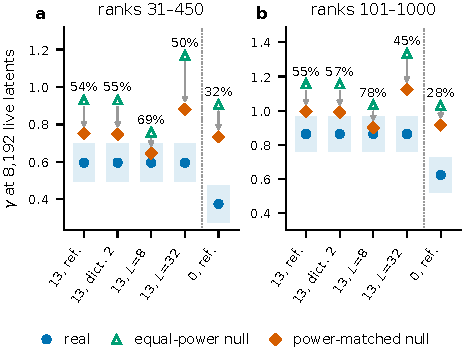
\includegraphics[width=0.8\textwidth]{fig13_pmatch_r2.pdf}
\caption{The power-matched settings in absolute terms, Gemma-2-2B, $k=40$, 8,192 live latents. For each setting: real (three-seed mean), the equal-power null and the power-matched null at the same $(M, L)$, each FVU-matched. Arrows show the effect of matching atom power; numbers give the share of the real-to-null gap it closes. Shading: within 0.10 of real, the decision rule's ``closed'' band. Labels give the layer and the setting (ref.: $M=8{,}192$, $L=16$); ``dict.\ 2'' is a second dictionary draw with new token streams. Starred settings show three-seed values as in Table~\ref{tab:pmatch2} (power-matched mean with its seed sd bar, smaller than the marker, and seed dots; equal-power mean of two seeds, three at 32,768 atoms; shares in bold); the others are the first run, with one seed per null and the equal-power null's seed 0. At 32,768 atoms the power-matched null needed $\rho=0.34$ and its equal-power comparator $\rho=0$. Real is the same in the first five columns.}
\label{fig:pmatch}
\end{figure}

\begin{table}[!htb]
\centering
\caption{Power concentration of the trained SAEs, measured on 1M tokens: share of latent power in the top 10 latents and the top 1\% of latents. Power-matched rows with three seeds give the seed mean.}
\label{tab:manip}
\small
\begin{tabular}{l rr rr}
\toprule
 & \multicolumn{2}{c}{layer 13} & \multicolumn{2}{c}{layer 0} \\
\cmidrule(lr){2-3}\cmidrule(lr){4-5}
SAE & top 10 & top 1\% & top 10 & top 1\% \\
\midrule
real (seed 0) & 0.18 & 0.35 & 0.03 & 0.11 \\
equal-power null & 0.21 & 0.48 & 0.14 & 0.27 \\
power-matched null, reference (three seeds) & 0.20 & 0.53 & 0.14 & 0.29 \\
power-matched null, $L=8$ / $L=32$ & 0.21 / 0.21 & 0.56 / 0.52 & -- & -- \\
power-matched null, $M=32{,}768$, $\rho=0.34$ (three seeds) & 0.23 & 0.52 & -- & -- \\
power-matched null, $M=32{,}768$, $\rho=0$ (FVU 0.083) & 0.09 & 0.22 & -- & -- \\
\bottomrule
\end{tabular}
\end{table}

\textbf{A variant not run.} We also tried matching each latent's power together with its Rayleigh quotient $w^\top\Sig w/(\mathrm{tr}\,\Sig/d)$, so that the dictionary would reproduce how strongly the real latents line up with $\Sig$. Locally the iteration did not approach its targets under any assignment rule: after 25 rounds the power errors were 2--8 in log and the quotient errors 0.3--0.6 in $\log_{10}$. The constraint $A^\top A=\Sig$ fixes the power-weighted second moment of the directions, and the real latents do not decompose $\Sig$: their powers sum to 0.39 of the variance at layer 13. At layer 0 they sum to 0.95 of $\mathrm{tr}\,\Sig$ for the 10M-token $\Sig$ from which the nulls are built, and to 0.99 of the variance of the 1M tokens on which power was measured; at layer 13 the two estimates agree. The variant stayed out of the run, so the effect of power together with the measured alignment is untested.

\textbf{Feature power on the real SAEs.} The real seed-0 SAEs at layers 13 and 0 were retrained with their encoders from the original configuration (FVU 0.2875 against 0.2870, and 0.1131 against 0.1132; $\gamma$ within 0.011), and power was measured on the last 1M cached tokens. At layer 13 the top 10 latents carry 18\% of the power at a median Rayleigh quotient of 43, power and quotient correlate at Spearman 0.58, and the latents outside the top 1\% have a median quotient of 3.0. At layer 0 the top 10 carry 3\%, the effective number of latents is 22\% of the live ones, and the body's median quotient is 1.4. The equal-power null SAEs have negative correlations between power and quotient ($-0.64$ and $-0.69$) and bodies with median quotients of 1.5 and 2.2, so they pass part (b) of the head/body rule and fail part (a), because power weighting does not raise their bulk $\gamma$.

\section{The ladder: details}
\label{app:ladder}

\textbf{Datasets.} Each dataset is 10M tokens of the Pile stream used throughout (shuffle seed 0, 1,024-token rows, BOS dropped), tokenised with the Gemma-2-2B tokenizer, with $\Sig$ accumulated in float64. embT is the trained input embedding as the model feeds it to block 0 (embedding row times $\sqrt{d}=48$), read with a hook before block 0. embR replaces the embedding matrix by i.i.d.\ $N(0,s^2)$ entries with $s=0.0375$, the RMS of the trained matrix (generator seed 4321), and applies the same scaling. randL0 and randL13 come from one Gemma-2-2B built from its published configuration with the library's default initialisation (\texttt{transformers} 5.23.0, \texttt{torch.manual\_seed(1234)}, float32 on the CPU, then cast to bf16 like the trained model): every linear and embedding weight is $N(0, 0.02^2)$, the padding row is zero, and the RMSNorm weights are zero, which in Gemma's $(1+w)$ parameterisation is unit gain. The initialisation is not scaled with depth, so the residual stream grows across blocks; another scheme could give a different block-13 dataset. The block-13 collection rebuilt the model with the same seed and checked that its embedding and block-0 weights hash to the block-0 collection's.

\textbf{$\Sig$ and fit quality.} Table~\ref{tab:ladder_detail} gives $\Sig$'s top-1 and top-10 eigenvalue shares, its participation ratio and its slopes in the bulk windows. No dataset met the job's degeneracy test (top-1 share above 0.99, or fewer positive eigenvalues than $\min(d,1000)$); all have 2,304 positive eigenvalues. The trained embeddings are dominated by one direction (23\% of the variance, participation ratio 17); the random-model datasets are less concentrated than trained Gemma at the same layer. $\Sig$'s bulk log-log fits have $R^2\ge 0.99$ everywhere. The decoder clouds fit less well in two places. At randL13 both nulls' spectra bend inside each bulk window: over the lower and upper halves of ranks 31--450 (split near rank 118) the equal-power null's $\gamma$ is 0.81 and 1.94, and over the halves of ranks 101--1000 (split near rank 318) 1.47 and 3.24; the worst fit has $R^2=0.93$. The real randL13 SAEs fit with $R^2\ge 0.98$. On the embeddings the real SAEs' clouds bend the other way, flat at the low ranks of each window ($\gamma$ 0.08 and 0.29 over the halves of ranks 31--450 on embR), with $R^2$ down to 0.94; the nulls there fit with $R^2\ge 0.994$. On the trained model every cloud fits with $R^2\ge 0.96$.

\begin{table}[!htb]
\centering
\caption{Ladder datasets and their trained counterparts. $\Sig$: top-1 and top-10 eigenvalue shares and participation ratio (PR), and $\Sig$'s slope with the $R^2$ of its log-log fit in the two bulk windows. Cloud fit: smallest $R^2$ over the real, equal-power and power-matched decoder clouds (fixed-$n$ mean spectrum) in ranks 31--450 / 101--1000. Live latents: smallest count among the real, equal-power and power-matched SAEs. Top-1\% power: share of latent power on the top 1\% of latents for the real seed-0 SAE, of atom power for the power-matched dictionary, and of latent power for the SAE trained on it.}
\label{tab:ladder_detail}
\footnotesize
\setlength{\tabcolsep}{2.5pt}
% generated by paper/figures/make_fig_ladder.py from results/r2/ladder_summary.json and ladder_extra.json
\begin{tabular}{l rrr cc c c c}
\toprule
 & \multicolumn{3}{c}{$\Sigma$} & \multicolumn{2}{c}{$\Sigma$ slope ($R^2$)} & cloud fit & live latents & top-1\% power \\
\cmidrule(lr){2-4}\cmidrule(lr){5-6}
dataset & top-1 & top-10 & PR & 31--450 & 101--1000 & min $R^2$ & $R$/$Z$/$N$ (min) & real/dict./null SAE \\
\midrule
embT (Gemma emb.) & 0.229 & 0.399 & 17 & $-0.822$ (0.998) & $-0.767$ (1.000) & 0.980/0.959 & 16{,}382/9{,}079/11{,}397 & 0.22/0.21/0.48 \\
embR (random emb.) & 0.032 & 0.197 & 169 & $-0.877$ (0.992) & $-0.765$ (1.000) & 0.942/0.944 & 16{,}384/12{,}188/12{,}770 & 0.11/0.10/0.41 \\
Gemma, block 0 & 0.048 & 0.165 & 195 & $-0.728$ (1.000) & $-0.713$ (1.000) & 0.986/0.962 & 16{,}384/13{,}368/13{,}305 & 0.11/0.10/0.30 \\
randL0 & 0.029 & 0.146 & 273 & $-0.758$ (0.998) & $-0.744$ (0.999) & 0.964/0.962 & 16{,}384/14{,}199/15{,}382 & 0.22/0.22/0.39 \\
Gemma, block 13 & 0.063 & 0.233 & 111 & $-0.750$ (0.995) & $-0.705$ (1.000) & 0.993/0.978 & 16{,}242/14{,}572/14{,}470 & 0.35/0.32/0.53 \\
randL13 & 0.040 & 0.151 & 234 & $-0.722$ (0.999) & $-0.753$ (1.000) & 0.929/0.972 & 16{,}337/16{,}384/16{,}384 & 0.24/0.24/0.52 \\
\bottomrule
\end{tabular}

\end{table}

\textbf{Calibration.} The equal-power null starts at $\rho=0.3$ ($\rho=0$ when the target FVU is below 0.045), takes a Newton step with $dF/d\rho=0.65$, then secant steps, accepting the first run within 0.03 of the mean real FVU. embT: $\rho=0$ left FVU 0.012 against a target of 0.044, and $\rho=0.05$ gave 0.038. embR: $\rho=0.30$ gave 0.202 against 0.085, and $\rho=0.12$ gave 0.092. randL0: 0.228 at $\rho=0.30$ and 0.293 at 0.40 against 0.295. randL13: 0.236 at $\rho=0.30$ and 0.621 at 0.86 against 0.601. Each power-matched null started from its equal-power null's $\rho$ and matched at that first run: FVU 0.048, 0.114, 0.311 and 0.587. The embR value is 0.029 above its target, just inside the tolerance. The second seed of each equal-power null, at the accepted $\rho$, agreed with the first within 0.002 in FVU and 0.008 in bulk $\gamma$.

\textbf{Dense share at randL13.} The accepted $\rho=0.86$ is far above any value needed on the trained model (0.13--0.43), and the equal-power null's bulk $\gamma$ follows it: 1.00 and 1.11 at $\rho=0.30$, 1.45 and 2.65 at 0.86, while the real SAEs read 0.875 and 1.161. At $\rho=0.30$ the equal-power gap would have been 0.13 and $-0.05$. Our reading, not tested directly, is that an SAE codes a null that is 86\% Gaussian largely along $\Sig$'s leading directions, which would steepen its decoder spectrum past them; either way, the remainder at randL13 mostly measures how much Gaussian variance the null needs to be as hard to code as the data. The real randL13 SAEs also generalise less well than the others: on the last 1M cached tokens, half of which were training tokens, FVU is 0.51 against 0.60 on the held-out tokens, while on the other datasets the two agree within 0.002.

\textbf{Live latents and extra $k$.} The real $k=40$ SAEs have 16,337--16,384 live latents. The nulls' SAEs leave more latents dead on the embeddings (equal-power 9,079--9,162 on embT and 12,188--12,346 on embR; power-matched 11,397 and 12,770) than on randL0 (14,199--15,382) and randL13 (16,384); all are above the 8,192 used for scoring, so none is flagged. On both embedding datasets real SAEs with $k=4$ and $k=16$ (seed 0) read bulk $\gamma$ of 0.37 and 0.58 ($k=4$) and 0.32 and 0.57 ($k=16$) on embT, against 0.31 and 0.57 at $k=40$; and 0.21 and 0.50, and 0.20 and 0.48, on embR, against 0.19 and 0.46. Their FVU is 0.086 and 0.047 on embT and 0.093 and 0.092 on embR. The $k=4$ SAE on embT has 7,215 live latents and is scored on all of them; it enters no verdict.

\textbf{Power.} The power-matched dictionaries converged in 9, 5, 20 and 36 rounds (embT, embR, randL0, randL13) with a largest log power error of 0.020--0.029; their covariance matches $\Sig$ to a relative $3\times10^{-10}$ (embT) and $4$--$8\times10^{-13}$ (the others) in float64, and 1M samples from each generator to 0.011--0.019. The Spearman correlation between an atom's power and its Rayleigh quotient, the alignment forced by $\Sig$, is 0.11, 0.38, 0.49 and 0.80. As on the trained model, the SAE trained on each power-matched null concentrates its power more than the real SAE: its top 1\% of latents carry 0.48, 0.41, 0.39 and 0.52 of the power, against 0.22, 0.11, 0.22 and 0.24 for the real seed-0 SAE and 0.21, 0.10, 0.22 and 0.24 for the dictionary's atoms (trained layers 0 and 13: 0.30 and 0.53 against 0.11 and 0.35).

\textbf{Trained reference.} The rule compares with the trained model's first power-matched run (seed 0), as its script specifies. With the three-seed mean of Table~\ref{tab:pmatch2} instead, the trained remainder is 0.363 and 0.292 at layer 0 and 0.155 and 0.129 at layer 13, and the ratios become 1.51 and 1.32 (randL0) and 3.57 and 8.47 (randL13); no verdict changes. The additional analyses in this appendix (fit quality, half-window slopes, the three-seed reference) were made after seeing the results and do not alter the rule.

\section{The primary and top windows under the equal-power null}
\label{app:primary}

\begin{table}[!htb]
\centering
\caption{Real and equal-power null SAEs at eight layers of Gemma-2-2B in the reference setting ($k=40$, width 16,384; real three seeds, null two). $\rho$ is the null's dense share. Each $\gamma$ is a seed mean. The interval is a 90\% Welch interval from the seed spread, with 1.0--2.5 degrees of freedom. It lies inside $\pm 0.06$, a margin chosen after seeing the data, at layers 9, 13 and 17, and excludes zero at every layer but 17. The null's own dictionary has $\gamma=0.986$--1.000 in every window.}
\label{tab:matched}
\small
% generated by paper/figures/make_fig_null_r2.py from results/r2/runs_real.jsonl and runs_sparse2.jsonl
\begin{tabular}{r r c cc c cc}
\toprule
 & & FVU & \multicolumn{5}{c}{$\gamma$ at 8,192 live latents, real / sparse null} \\
\cmidrule(lr){4-8}
layer & $\rho$ & real / null & 4--50 & 11--150 & real $-$ null, 11--150 [90\%] & 31--450 & 101--1000 \\
\midrule
0 & 0.13 & 0.11/0.11 & 0.32/0.42 & 0.30/0.67 & $-0.365$ [$-0.478$, $-0.252$] & 0.38/0.91 & 0.62/1.03 \\
3 & 0.25 & 0.20/0.19 & 0.30/0.25 & 0.44/0.55 & $-0.109$ [$-0.151$, $-0.067$] & 0.64/0.93 & 0.72/1.04 \\
6 & 0.29 & 0.22/0.20 & 0.37/0.24 & 0.46/0.52 & $-0.058$ [$-0.073$, $-0.043$] & 0.69/0.92 & 0.79/1.05 \\
9 & 0.34 & 0.25/0.23 & 0.45/0.24 & 0.49/0.52 & $-0.028$ [$-0.033$, $-0.023$] & 0.64/0.93 & 0.81/1.10 \\
13 & 0.43 & 0.29/0.28 & 0.47/0.23 & 0.48/0.51 & $-0.030$ [$-0.041$, $-0.019$] & 0.60/0.93 & 0.86/1.16 \\
17 & 0.35 & 0.25/0.24 & 0.47/0.24 & 0.46/0.48 & $-0.014$ [$-0.055$, $+0.027$] & 0.52/0.88 & 0.75/1.12 \\
21 & 0.32 & 0.25/0.24 & 0.40/0.26 & 0.42/0.56 & $-0.144$ [$-0.183$, $-0.106$] & 0.45/0.95 & 0.65/1.10 \\
24 & 0.40 & 0.27/0.25 & 0.35/0.23 & 0.34/0.55 & $-0.207$ [$-0.214$, $-0.201$] & 0.41/0.95 & 0.66/1.12 \\
\bottomrule
\end{tabular}

\end{table}

\textbf{Primary window over layers.} Table~\ref{tab:matched} gives the eight-layer comparison. With three real and two null seeds, the 90\% Welch interval for real minus null lies inside $\pm 0.06$ at layers 9, 13 and 17, which would be a two one-sided test at the 5\% level if the margin had been fixed in advance. It was not. At layer 6 the point difference is $-0.058$ and the interval reaches $-0.073$. The null is steeper than real at every layer, so the difference has a consistent sign.

\textbf{Primary window over $k$.} At layer 13 the null's $\gamma$ is within 0.08 of real's at every $k\ge 24$ and within 0.04 at $k\ge 32$ (Figure~\ref{fig:matched}f, Figure~\ref{fig:k}), but it falls faster with $k$: 1.44 times as fast per doubling over $k=24$--128, and 1.59 times over $k=16$--128. At $k=8$ and 16 the null is steeper (0.87 against 0.74, and 0.81 against 0.65). FVU is matched only at $k=40$; it stays within 0.023 of real's for $k\ge 16$ and is 0.09 higher at $k=8$.

\textbf{Dependence on $\rho$.} In the calibration runs the null's ranks 11--150 $\gamma$ falls as $\rho$ rises at every layer, from 0.69--0.89 at $\rho=0$, so the middle layers agree only near the calibrated share. That share assumes the variance a width-16,384 SAE leaves uncoded is dense Gaussian; if it is sparse structure beyond the SAE's width, a lower $\rho$ would be appropriate.

\textbf{Top window.} In ranks 4--50 the sign of the difference depends on $\rho$. At layer 13 the null's $\gamma$ is 0.56, 0.39 and 0.23 at $\rho=0$, 0.13 and 0.43 (the calibrated value), and real's is 0.47. At layers 3--24 real lies between the null at $\rho=0$ and the calibrated null, and at layer 0 it is below both. At the calibrated $\rho$ real is steeper than the null at layers 3--24, by 0.05 to 0.23, and at layer 13 at every $k$ and under every generator setting.

\textbf{Reading (v).} Before the equal-power runs we fixed the reading that the three signatures separating real from Gaussian-null SAEs (a flatter bulk, a mid-stack top-window profile, and the decline of $\gamma$ with $k$) would also separate real from this null. Under the window rule it is contradicted (Appendix~\ref{app:sparse2}).

\textbf{Resynthesis.} A separate control asked whether the second moments of a trained dictionary carry the decline of $\gamma$ with $k$. Data resynthesised from the codes of the Gemma Scope 65k SAE at layer 12 on directions drawn from a Gaussian with the decoder rows' covariance retains 0.53--0.79 of the decline seen on the decoder's own rows, so the pre-specified reading is mixed; over $k=16$--128, a range chosen afterwards, it retains 0.45 in ranks 11--150 (Appendix~\ref{app:resynth}).

\begin{figure}[!htb]
\centering
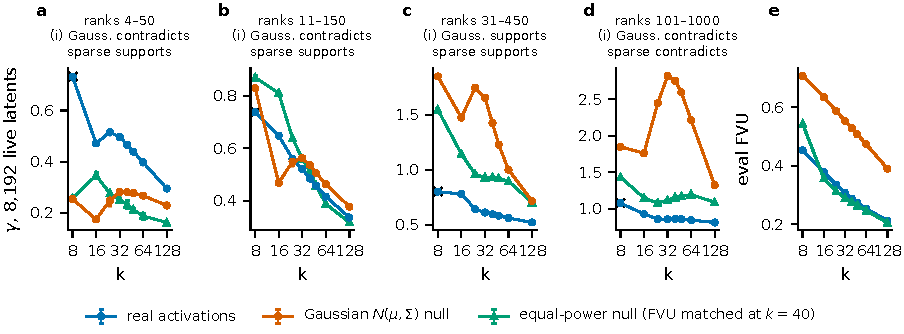
\includegraphics[width=\textwidth]{fig9_k_sweep_r2.pdf}
\caption{$\gamma$ against $k$ at layer 13 for real (blue) and Gaussian-null (orange) SAEs (width 16,384, 8,192 live latents; mean $\pm$ sd over three seeds, dots are seeds; $\Sig$ from the 10M training tokens; $k=40$ from the eight-layer runs), and for the equal-power sparse null (green, two seeds, FVU matched to real at $k=40$). Panel titles give reading (i), that a null declines as steadily as real over $k=16$--128, for each null. In ranks 11--150 the real $\gamma$ falls steadily while the Gaussian null's falls in one step between $k=8$ and 16 and then rises and falls; in ranks 4--50 it does not decline. In ranks 31--450 the Gaussian null declines 4.3 times faster than real. $\times$: the real $k=8$ SAEs have fewer than 8,192 live latents (6,219--6,507). (e) Eval FVU.}
\label{fig:k}
\end{figure}

\clearpage
\section{Generator settings and the GPT-2 null}
\label{app:robust}

\begin{table}[!htb]
\centering
\caption{Generator settings of the equal-power null at layers 13 and 0 of Gemma-2-2B ($k=40$, width 16,384, one seed), each with $\rho$ calibrated to the real SAE's FVU (targets 0.288 and 0.114). $M$: atoms; $L$: active atoms per token. $^{*}$: the reference setting (seed-0 run of Table~\ref{tab:matched}). $^{o}$: overflow setting, in which the dense remainder is replaced by a second dictionary of 65,536 atoms with 64 active per token and $\rho$ is its variance share. $\dagger$: FVU not matched at $\rho=0$, excluded by the pre-specified rule. Real is the three-seed mean.}
\label{tab:robust}
\small
% generated by paper/figures/make_fig_null_r2.py from results/r2/runs_robust.jsonl, runs_sparse2.jsonl and runs_real.jsonl
\begin{tabular}{r r r r r rrrr}
\toprule
 & & & & & \multicolumn{4}{c}{real $-$ null $\gamma$} \\
\cmidrule(lr){6-9}
layer & $M$ & $L$ & $\rho$ & FVU & 4--50 & 11--150 & 31--450 & 101--1000 \\
\midrule
13 & 8192$^{*}$ & 16 & 0.43 & 0.275 & $+0.22$ & $-0.03$ & $-0.33$ & $-0.29$ \\
 & 4096 & 16 & 0.43 & 0.273 & $+0.27$ & $+0.02$ & $-0.30$ & $-0.23$ \\
 & 8192 & 8 & 0.43 & 0.265 & $+0.30$ & $+0.13$ & $-0.16$ & $-0.17$ \\
 & 8192 & 16$^{o}$ & 0.43 & 0.276 & $+0.24$ & $-0.03$ & $-0.34$ & $-0.29$ \\
 & 8192 & 32 & 0.42 & 0.293 & $+0.15$ & $-0.19$ & $-0.57$ & $-0.47$ \\
 & 32768 & 16 & 0.00 & 0.309 & $+0.26$ & $+0.07$ & $-0.16$ & $-0.14$ \\
\midrule
0 & 8192$^{*}$ & 16 & 0.13 & 0.112 & $-0.09$ & $-0.35$ & $-0.53$ & $-0.41$ \\
 & 4096 & 16 & 0.14 & 0.115 & $-0.12$ & $-0.48$ & $-0.50$ & $-0.27$ \\
 & 8192 & 8 & 0.14 & 0.112 & $-0.02$ & $-0.28$ & $-0.43$ & $-0.36$ \\
 & 8192 & 32 & 0.12 & 0.121 & $-0.20$ & $-0.49$ & $-0.65$ & $-0.52$ \\
 & 32768$^\dagger$ & 16 & 0.00 & 0.354 & $+0.06$ & $-0.21$ & $-0.41$ & $-0.38$ \\
\bottomrule
\end{tabular}

\end{table}

\textbf{Gemma-2-2B.} Besides the reference setting we trained null SAEs at layers 13 and 0 with $(M,L)$ equal to (4096, 16), (32768, 16), (8192, 8) and (8192, 32), and at layer 13 with the overflow setting (Table~\ref{tab:robust}). One setting could not be used: at layer 0 the null with 32,768 atoms already leaves FVU 0.354 at $\rho=0$, far above the target of 0.114, so no dense share can match it. The other eight matched, with $\rho$ from 0 to 0.43 and FVU within 0.023 of the target. Real decoders are flatter than the null in both bulk windows at all eight, by 0.14 to 0.65. The gap is smallest, 0.137 in ranks 101--1000, with 32,768 atoms at layer 13, the setting that needed no dense share; the rule fixed before the run asked for at least 0.15 everywhere, so it calls the result partial rather than robust. The primary window is more sensitive. At layer 13 real minus null in ranks 11--150 is $+0.02$ with 4,096 atoms, $-0.03$ in the overflow setting, $+0.07$ with 32,768 atoms, $+0.13$ with 8 active atoms and $-0.19$ with 32, so the number of active atoms moves it most. In ranks 4--50 real is steeper than the null at all five layer-13 settings, by 0.15 to 0.30, and at layer 0 the null is steeper than real in ranks 11--150 at every matched setting, by 0.28 to 0.49.

\begin{figure}[!htb]
\centering
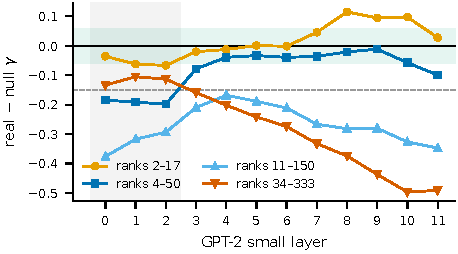
\includegraphics[width=0.7\textwidth]{fig12_gpt2_codable_r2.pdf}
\caption{GPT-2 small: real minus equal-power null $\gamma$ at $k=32$ over the 12 layers (null one seed in the reference setting; real one seed, two at layer 6), windows scaled to $d=768$ (ranks 4--50 primary). Grey columns: layers 0--2, where the null's SAE reached the real FVU at $\rho=0$. Green band: $\pm 0.06$. Dashed line: $-0.15$, the bulk bar of the pre-specified rule.}
\label{fig:gpt2codable}
\end{figure}

\textbf{GPT-2 small.} We trained the reference null at all 12 GPT-2 layers at $k=32$, calibrated by the same rule (Figure~\ref{fig:gpt2codable}). All 12 matched, with FVU within 0.019. At layers 0--2 the null's SAE already reaches the real FVU (0.03--0.04) at $\rho=0$; elsewhere $\rho$ is 0.09--0.36. In the bulk, real is 0.17--0.38 below the null at every layer in ranks 11--150 and 0.11--0.50 below in ranks 34--333. In the second window it misses 0.15 at the three layers that needed no dense share, the same pattern as the 32,768-atom setting on Gemma, so the bulk statement only partly replicates (the rule asked for 0.15 at 90\% of layers in both windows). In the primary window (ranks 4--50) the null tracks real at layers 4--10, within 0.012--0.058, so it agrees within 0.06 at two thirds or more of the interior layers 3--8 and at no more than one of the end layers 0, 1, 10 and 11, and the primary-window statement replicates. In the top window (ranks 2--17) real is steeper at six layers and flatter at six, so the mid-stack top-window signature seen on Gemma does not carry over.

\section{Does $\gamma$ predict SAE quality?}
\label{app:quality}

\textbf{Samples.} (A) 52 Gemma Scope residual SAEs whose $\gamma$ we had already computed and which have public SAEBench results: Gemma-2-2B layers 5, 12 and 19 at 16k and 65k (five each) and layer 12 at 1M (two); Gemma-2-9b 16k at layers 9, 20 and 31 (6, 8 and 6). (B) The 42 SAEs of SAEBench's width-4,096 suite on Gemma-2-2B layer 12 (seven architectures at six sparsities), whose decoders we downloaded and scored exactly as the Gemma Scope SAEs. (C) Our own 51 real-data TopK SAEs within 18 (layer, $k$) cells, for which only FVU and the dead fraction exist.

\textbf{Plan, fixed before the analysis.} Seven SAEBench metrics (CE-loss recovery, explained variance, absorption, sparse-probing top-1 accuracy, SCR and TPP at 20 latents, autointerp). Model~1: metric on layer fixed effects, $\log_2\Lz$, $(\log_2\Lz)^2$ and $\log_2$ width; Model~2 adds FVU and is the decision model for the five metrics other than reconstruction. Effect size: partial correlation of $\gamma$ with the metric. Intervals from a two-stage cluster bootstrap (2,000 replicates), $p$-values from 10,000 within-cluster permutations, Holm correction over 7 metrics $\times$ 4 windows per sample. $\gamma$ ``predicts'' a metric if the primary-window test is Holm-significant, the sign agrees in at least two other windows and in every leave-one-cluster-out refit, and $|r|\ge 0.3$. A practical claim needs such a metric outside reconstruction that also has the same sign at $p<0.05$ in the other sample. Two corrections were made after the first run: whitened-input runs were removed from sample C, as the plan's ``real-data SAEs'' requires, and sample B uses SAEBench's newer absorption field because the older one is absent from that release.

\textbf{Results.} Layer, $\Lz$ and width explain 94--97\% of $\gamma$'s variance in sample A and 40--89\% in sample B. In A only CE-loss recovery passes (partial $r=-0.49$, Holm $p=0.003$); it is a reconstruction metric, so the practical criterion is not met. The pre-specified robustness check that gives each layer its own $\Lz$ slope moves it to $+0.20$ and shrinks every Holm-significant cell in A to $|r|\le 0.36$. In B nothing passes, and adding architecture fixed effects reduces the CE-loss association to $-0.20$. In C, seed-to-seed $\gamma$ does not track FVU or the dead fraction: $|r|\le 0.27$ in the top windows, up to 0.49 (dead fraction) in the bulk windows, and no Holm-adjusted $p$ below 0.5. No primary-window interval lies inside $(-0.3, 0.3)$, so none of this is a clean null: with 6--7 clusters the intervals are 0.9 to 1.7 wide. Post hoc, $\gamma$ in ranks 101--1000 is positively associated with autointerp after $\Lz$ and FVU in both samples ($r=+0.79$ in B, $+0.35$ in A); this was not a pre-specified window, is one of 28 tests per sample, and would need its own pre-specified test on a new sample.


\section{Methods}
\label{app:methods}

\textbf{Data and activations.} Gemma-2-2B residual stream after each block (\texttt{resid\_post}), on the uncopyrighted subset of the Pile, context 1,024, beginning-of-sequence position dropped. Pythia-70m layer 3 used context 256. For our Gemma SAEs we cached 10M tokens per layer and held out the last 0.5M for evaluation; $\mu$ and $\Sig$ for both nulls and for $\gamma$ of our SAEs come from this cache. Figure~\ref{fig:l0}, Section~\ref{sec:l0} and Appendix~\ref{app:li} use the 1M-token $\Sig$.

\textbf{Rank windows in code.} Windows are stored as 0-based slices of the sorted eigenvalues: \texttt{(3, 50)}, \texttt{(10, 150)}, \texttt{(30, 450)} and \texttt{(100, 1000)} are ranks 4--50, 11--150, 31--450 and 101--1000; \texttt{(0, 100)} is ranks 1--100. For GPT-2 small ($d=768$) each bound is scaled by $d/2{,}304$, giving ranks 2--17, 4--50 (primary), 11--150 and 34--333; for Gemma-2-9b ($d=3{,}584$) the scaled windows are ranks 6--78, 17--233 (primary), 48--700 and 157--1556.

\textbf{Our SAEs.} TopK SAEs with an auxiliary TopK loss on dead latents ($k_{\mathrm{aux}}=512$, coefficient $1/32$, a latent is dead after 2M tokens without firing), unit-norm decoder rows with the parallel gradient component removed, Adam with learning rate $2\times10^{-4}\sqrt{16384/n}$ for width $n$ and linear decay over the last 20\% of steps, batch 4,096 tokens, inputs scaled so that $\mathbb{E}\|x\|^2=d$ with the same constant for every condition. Null samples are drawn fresh for every batch (28.5M distinct samples); real data are 9.5M tokens seen three times. Scrambled data permute each coordinate independently across tokens. In the three-layer set (Tables~\ref{tab:null} and \ref{tab:65k}) seed-to-seed sd at $k=40$ is at most 0.013 in raw slope (0.009 for real and Gaussian). In the eight-layer runs it is at most 0.009 (real) and 0.015 (Gaussian) at 8,192 live latents, and in the layer-13 $k$ sweep at most 0.019 in $\gamma$. FVU is measured on the 0.5M held-out tokens. Fixed-count scoring draws 8,192 live latents four times (seed $100k+s$ for SAE seed $s$) and averages the slopes; the three-layer set is scored on all live rows. Where fewer than 8,192 latents are live we use all of them and mark the point.

\textbf{Whitened SAEs.} At layer 12 the inputs are $x_w = (\Sig+\epsilon I)^{-1/2}(x-\mu)$ with $\epsilon = 10^{-3}$ times the mean eigenvalue of $\Sig$, and $\mu,\Sig$ from all 10M cached tokens. Decoder rows $w$ are mapped back as $u = w(\Sig+\epsilon I)^{1/2}/\|w(\Sig+\epsilon I)^{1/2}\|$ and scored against $\Sig$ like every other SAE. The isotropic reference draws as many directions as the SAE has live latents, isotropically in whitened space, and maps and scores them the same way. The control SAE is trained on the same tokens unwhitened. The reading was: whitened decoders are isotropic in a window if the mapped $\gamma$ is within 0.05 of the isotropic reference at $k=16$, 40 and 128, and not if it differs by more than 0.05 and two standard errors at all three.

\textbf{GPT-2 small.} \texttt{resid\_post} of all 12 blocks (layer 11 before the final layer norm), 10M Pile tokens per layer cached as for Gemma, last 0.5M held out, the same SAE recipe at width 16,384; one seed per layer at $k=32$ (two at layer 6), and two seeds at layer 6 with $k \in \{8,16,32,64,128\}$.

\textbf{Local SAEs.} The Pythia-70m SAEs of Appendix~\ref{app:gregime} (layer 3, $k=32$, widths 1,024, 4,096 and 16,384, three seeds each for real, Gaussian and scrambled data) make one pass over 15M tokens and are evaluated on 1M further tokens; their $\Sig$ comes from the 20M-token activation cache they are drawn from. The Gemma-2-2B width-4096 $k=40$ SAEs of Appendix~\ref{app:regime} are trained on 0.8M tokens at layer 12 (real and Gaussian, $\Sig$ from the 1M-token cache) and on 3M Gaussian samples at layers 0, 3, 7, 13, 17, 21 and 24 ($\Sig$ from 200,508 tokens), and evaluated on 0.2M tokens. The same optimiser settings apply.

\textbf{Gemma Scope SAEs.} Decoder rows of the 288 \texttt{gemma-scope-2b-pt-res} SAEs (all 26 layers at widths 16k and 65k, plus layer 12 at 32k, 131k, 262k, 524k and 1M), all rows, unit norm. Our reproduction of \citet{li2025geometry} (65k SAEs at layers 0, 12 and 24) gives $-0.2383$, $-0.4684$ and $-0.2545$, within 0.02\% of their values; centring and row normalisation change the slope by at most 0.0008. We measured $\Lz$ on 1M tokens for the 22 of the 28 layer-12 SAEs whose encoder we had. The matched-$\Lz$ layer profiles interpolate each layer's slope linearly in $\log \Lz$ between the two SAEs that bracket the target. For Gemma-2-9b we analyse 96 \texttt{gemma-scope-9b-pt-res} 16k SAEs: every available $\Lz$ at layers 9, 20 and 31, and the $\Lz$ nearest 40 and 70 elsewhere, with $\Sig$ from 1M Pile tokens.

\textbf{Correlations across layers.} Effective sample size from Bartlett's formula with lags up to $n/4$, a Fisher-$z$ interval at that size, 10,000 phase-randomised surrogates of the decoder series, and all 25 circular shifts (resolution $1/26$). We quote the effective-size interval as the conservative one. Partial correlations in Appendix~\ref{app:cluster} are Spearman, with the same surrogates.

\textbf{$\Sig$-decoder correlation across layers.}
\label{app:corr}
For the correlation of Section~\ref{sec:l0} at $\Lz=40$ in ranks 11--150, Bartlett's effective sample size is 6.5, which gives a 95\% interval of $[0.50, 0.99]$; phase-randomised surrogates give $p<10^{-4}$ and circular shifts $p=0.038$, the smallest value that 26 shifts can produce. The other windows tell a similar but weaker story. In the top windows at $\Lz=40$ and 70, at both widths, $r$ is 0.75--0.92 with effective sizes of 6.4--7.0, so the intervals are wide (their lower ends run from $-0.01$ to 0.50), although the phase-surrogate $p$ stays at or below 0.024. In ranks 31--450 the correlation is $r=0.81$ (16k) and 0.76 (65k) at $\Lz=40$, with surrogate $p$ of 0.021 and 0.037, and it weakens to $p=0.051$ and 0.058 at $\Lz=70$. In ranks 101--1000 the surrogate $p$ is 0.068--0.127. By $\Lz=140$ the correlation in ranks 11--150 has fallen to 0.37 ($p=0.60$). Under the rule we fixed in advance (the primary window plus two others, tested by phase surrogates) the correlation therefore passes at $\Lz=20$ and 40 and falls just short at 70, where Bartlett's effective-size test would pass ($p=0.031$ and 0.028 in ranks 31--450). At $\Lz=20$, 11 layers at 16k and 17 at 65k have Gemma Scope SAEs that bracket it. The correlation is observational: the training objective could pass $\Sig$'s shape to the decoder, or both could reflect depth-dependent structure in the activations.

\textbf{$\Sig$ estimation.} At layer 12, two halves of the 1M-token sample split by document give slopes within 0.003 of each other in every window. The first 200k tokens alone give bulk slopes steeper by 0.08 (ranks 31--450) and 0.12 (ranks 101--1000), so we use 1M tokens for every Gemma Scope $\Sig$. At the nine layers where we also have the 10M-token $\Sig$ of our SAEs (0, 3, 6, 9, 12, 13, 17, 21 and 24; a different sample of the same corpus), the two slopes differ by at most 0.034 in ranks 4--50, 0.029 in 11--150, 0.020 in 31--450 and 0.046 in 101--1000. In ranks 101--1000 the 1M-token slope is the steeper one at all nine layers, by 0.008 to 0.046, most at layers 0, 21 and 24.

\section{Live-count bias}
\label{app:live}

On 22 layer-12 Gemma Scope SAEs with up to 13.9\% dead rows, all-row and live-row slopes differ by at most 0.003 in ranks 11--150 and 0.013 in ranks 101--1000. The effect is larger in TopK SAEs with many dead rows. On local layer-12 TopK SAEs trained on PCA projections of the activations (width 8,192, $k=8$), all-row and live-row slopes differ by 0.025 in ranks 11--150 with 11\% of rows dead, and by up to 0.09 in ranks 11--150 and 0.22 in ranks 101--1000 with 33--42\% dead. A two-seed sweep at layer 13 with the same recipe went down to $k=1$, where 60--96\% of real rows (at $k \le 8$) and 90--97\% of Gaussian-null rows (at $k \le 4$) are dead; real minus null $\gamma$ in ranks 11--150 was $-0.21$, $-0.40$ and $-0.41$ at $k=1$, 2 and 4, on clouds whose live counts differ by a factor of 1.5 to 2.4. The calibration below is what makes such values comparable at all, and is why the main-text runs are scored at a fixed live count.

We simulated unit-normalised Gaussian clouds whose covariance is $\Sig_{13}^{g}$ ($\Sig$ at layer 13 raised to a true exponent $g$), with $n$ points, six draws each (sd $\le 0.01$), and measured $\gamma$ in ranks 11--150 (Table~\ref{tab:live}). A finite cloud pulls high $\gamma$ down and pushes $\gamma$ near zero up; an isotropic cloud of 16,384 unit vectors measures $\gamma=0.054$. Inverting this calibration at each SAE's live count (grid step 0.2, two draws) gives model-based corrected values: the real $k=1$ value moves from 1.034 (672 live latents) to 1.25, the real fit over $k=1$--128 from $1.016-0.094\log_2 k$ to $1.180-0.115\log_2 k$, and the Gaussian null at $k \le 4$ to 1.36--1.47. These corrections assume a Gaussian cloud with covariance a power of $\Sig$. Real decoder clouds only approximate one (Appendix~\ref{app:matrix}), and the Gaussian null's decoders are closer to one than real decoders are (Appendix~\ref{app:gregime}). We do not use the corrected values for any claim in the main text.

The bias differs by window. Repeating the simulation at $n=8{,}192$ (two draws, $\Sig$ from the 10M-token training cache at layer 13) gives measured $\gamma$ of 0.97, 0.96, 0.96 and 1.08 in ranks 4--50, 11--150, 31--450 and 101--1000 for a true exponent of 1, and 0.45, 0.41, 0.45 and 0.65 for a true exponent of 0.5. The ranks 11--150 values reproduce Table~\ref{tab:live} to within 0.002. In ranks 101--1000 a cloud reads high, by 0.08 at $g=1$ and 0.15 at $g=0.5$, so the bulk $\gamma$ of both the equal-power null SAEs (1.03--1.16) and the real SAEs should not be read as absolute exponents. All main-text comparisons are made at this $n$.

\begin{table}[!htb]
\centering
\caption{Measured $\gamma$ (ranks 11--150) of simulated clouds with true exponent $g$ and $n$ points, $d=2{,}304$.}
\label{tab:live}
\small
\begin{tabular}{l rrrrr}
\toprule
true $g$ & $n=672$ & 2,000 & 4,786 & 8,192 & 16,384 \\
\midrule
0 & 0.183 & 0.123 & 0.089 & 0.071 & 0.054 \\
0.5 & 0.289 & 0.319 & 0.376 & 0.414 & 0.450 \\
1.0 & 0.741 & 0.861 & 0.928 & 0.953 & 0.974 \\
1.25 & 1.027 & 1.137 & 1.192 & 1.213 & 1.228 \\
\bottomrule
\end{tabular}
\end{table}

\section{The equal-power sparse null: details}
\label{app:sparse2}

\textbf{Generator.} Each of the $M=8{,}192$ sources is active independently with probability $p=16/M$, so 16 are active per token on average. An active source takes the value $c|z|$ with $z$ standard normal and $c$ set so that each source has unit variance; values are one-signed so that a ReLU latent can code a source without a second latent for the other sign. The atoms are the rows of $A=R\,\Sig^{1/2}$, where $R$ is a random $M \times d$ matrix with orthonormal columns, and the dense remainder is $\sqrt{\rho}\,g$ with $g \sim N(0,\Sig)$, so the covariance is $\Sig$ for every $\rho<1$. $\mu$ and $\Sig$ are the 10M-token estimates of each layer. One data seed fixes the dictionary and the sample streams, and the SAE seed sets only the initialisation. Width, number of samples (fresh for every batch), passes and scoring are as for the other SAEs. At $k=40$ the SAEs have 13,368 to 14,686 live latents, so all are scored at the fixed 8,192. The dictionary itself, scored as a cloud of 8,192 unit rows, has $\gamma=0.986$ to 1.000 in every window at every layer.

\textbf{Calibration.} The target is the mean eval FVU of the three real $k=40$ SAEs at the layer. The first run uses $\rho=0$ (FVU 0.013--0.016 at the eight layers). The second uses a quarter of the linear interpolation between that FVU and the Gaussian null's, and later runs take secant steps; a run is accepted when its FVU is within 0.03 of the target, and at most four steps are allowed. Every layer was accepted at its third run, with $\rho$ as in Table~\ref{tab:matched}. The two earlier runs per layer (16 SAEs, one seed) are not part of the main comparison; they give the null at $\rho=0$ and at an intermediate $\rho$ (0.04--0.13, FVU 0.048--0.097) used in Section~\ref{sec:equal} and Appendix~\ref{app:primary}. At layer 13 the same $\rho$ is used at every $k$, so FVU is matched only at $k=40$.

\textbf{Equivalence in ranks 11--150.} For each layer we take the seed means of $\gamma$ (each seed's value is itself a mean over four draws of 8,192 live latents), their difference, and its standard error $\sqrt{s_R^2/3 + s_N^2/2}$. The 90\% interval uses Welch's $t$ with Satterthwaite's degrees of freedom, which are 1.0 to 2.5 because the null has two seeds. An interval inside $\pm 0.06$ is equivalent to two one-sided tests at the 5\% level. The margin was chosen after the results were known. The intervals are in Table~\ref{tab:matched}; the bulk-window intervals all lie below $-0.23$.

\textbf{Reading (v).} The reading was that the three signatures separating real from Gaussian-null SAEs would also separate real from the equal-power null. Each signature is tested only in windows where it separates real from the Gaussian null, by a ratio $f$ that compares the equal-power null's separation from real with the Gaussian null's: for the bulk, the summed real-minus-null slope difference over layers; for the top windows, the profile amplitude (largest interior-layer difference minus largest end-layer difference); for the decline with $k$, the difference in per-doubling slopes, in both $\gamma$ and raw slope. A window supports the reading if $f \ge 0.75$ and the original test still passes, and contradicts it if $f<0.5$. The mid-stack profile largely survives in the top windows ($f=0.85$ in ranks 4--50, 0.72 in ranks 11--150) and does not in the bulk ($f=0.44$ and 0.18). The decline with $k$ does not survive at all: $f$ is 0.09, $-0.99$ and $-0.19$ in ranks 4--50, 11--150 and 101--1000 (in ranks 31--450 the Gaussian null itself declines steadily, so the window does not apply). Under the window rule the reading is therefore contradicted. Run directly with the equal-power null in place of the Gaussian, the layer-profile test of Appendix~\ref{app:gprofile} passes in all four windows (maximum at layer 13 in ranks 4--50 and at layer 17 in ranks 11--150), and the $k$ test of Appendix~\ref{app:gk} finds a decline as steady as real's in ranks 4--50, 11--150 and 31--450 (per-doubling ratios 0.89, 1.59 and 1.62) and none in ranks 101--1000 ($+0.001$ against $-0.031$ for real). At $k=128$, $\gamma$ in the four windows is 0.29, 0.34, 0.52 and 0.81 for real and 0.16, 0.32, 0.70 and 1.09 for the equal-power null. Table~\ref{tab:sparse2} sets this null beside the Gaussian one.

\begin{table}[!htb]
\centering
\caption{Real, sparse-null and Gaussian-null SAEs at eight layers of Gemma-2-2B ($k=40$, width 16,384; real and Gaussian three seeds, sparse null two). Seed sd of the sparse null's $\gamma$ is at most 0.026.}
\label{tab:sparse2}
\small
% generated by paper/figures/make_fig_null_r2.py from results/r2/runs_real.jsonl and runs_sparse2.jsonl
\begin{tabular}{r r cccc c}
\toprule
 & & \multicolumn{4}{c}{$\gamma$ at 8,192 live latents: real / sparse null / Gaussian null} & FVU \\
\cmidrule(lr){3-6}
layer & $\rho$ & 4--50 & 11--150 & 31--450 & 101--1000 & real / sparse / Gauss. \\
\midrule
0 & 0.13 & 0.32/0.42/0.37 & 0.30/0.67/0.68 & 0.38/0.91/1.40 & 0.62/1.03/2.72 & 0.11/0.11/0.60 \\
3 & 0.25 & 0.30/0.25/0.36 & 0.44/0.55/0.64 & 0.64/0.93/1.42 & 0.72/1.04/2.50 & 0.20/0.19/0.56 \\
6 & 0.29 & 0.37/0.24/0.32 & 0.46/0.52/0.60 & 0.69/0.92/1.41 & 0.79/1.05/2.47 & 0.22/0.20/0.53 \\
9 & 0.34 & 0.45/0.24/0.33 & 0.49/0.52/0.60 & 0.64/0.93/1.39 & 0.81/1.10/2.62 & 0.25/0.23/0.54 \\
13 & 0.43 & 0.47/0.23/0.28 & 0.48/0.51/0.54 & 0.60/0.93/1.42 & 0.86/1.16/2.75 & 0.29/0.28/0.53 \\
17 & 0.35 & 0.47/0.24/0.29 & 0.46/0.48/0.56 & 0.52/0.88/1.40 & 0.75/1.12/2.79 & 0.25/0.24/0.56 \\
21 & 0.32 & 0.40/0.26/0.34 & 0.42/0.56/0.65 & 0.45/0.95/1.42 & 0.65/1.10/2.74 & 0.25/0.24/0.59 \\
24 & 0.40 & 0.35/0.23/0.31 & 0.34/0.55/0.61 & 0.41/0.95/1.45 & 0.66/1.12/2.76 & 0.27/0.25/0.52 \\
\bottomrule
\end{tabular}

\end{table}

\textbf{Generator settings and GPT-2.} The generator-settings run of Appendix~\ref{app:robust} and the GPT-2 null used the calibration routine above with one change, made from the 16 calibration points of the reference null before the run: the first guess after $\rho=0$ is $\rho_1 = 0.8\,(T-F_0)/(G-F_0)$, where $T$ is the target FVU, $F_0$ the FVU at $\rho=0$ and $G$ the Gaussian null's FVU. If $F_0 \ge T-0.03$ the setting keeps $\rho=0$, and it is unmatched if $F_0 > T+0.03$. At most three SAEs per Gemma setting and five per GPT-2 layer were allowed. In the overflow setting the second dictionary has 65,536 atoms $R_2\Sig^{1/2}$ with its own seed, 64 active per token and values $N(0,1)/\sqrt{p}$; on its own it is the first sparse null below, which a width-16,384 SAE cannot code. At layer 13, $M=32{,}768$ matched at $\rho=0$ (FVU 0.309 against 0.288); at layer 0 it did not (0.354 against 0.114). Real is the three-seed mean of the $k=40$ SAEs for Gemma-2-2B and the $k=32$ SAEs of Appendix~\ref{app:gpt2} for GPT-2. The null SAEs under the eight matched settings have mean Rayleigh quotients (Appendix~\ref{app:local}) of 1.7 to 3.5.

\textbf{The first sparse null.} It had $M=65{,}536$ sources with 64 active per token and normal values, and no dense share. In all 15 layer and $k$ settings where both were trained, its SAEs' FVU is within 0.001 of the Gaussian null's and its $\gamma$ within 0.012, 0.009, 0.018 and 0.059 in the four windows.

\section{Local analyses of the bulk gap}
\label{app:local}

All three analyses were run on CPU after the main runs, with one seed and no new training of real SAEs.

\textbf{Summary.} Three analyses look for structure in the bulk gap beyond what the nulls contain. The clearest is in $\Sig$'s eigenbasis. Rotated there, null decoder covariances are nearly diagonal, so their eigenvalues are essentially $\Sig$'s axes weighted. Real decoder covariances are not: their diagonal profile is flatter than the null's, and they carry substantial off-diagonal mass, with a coherence of 3.4--6.1 in ranks 31--450 against 0.28--0.56 for the equal-power null SAEs. A simple alternative, in which dictionaries spread power over $\Sig$'s eigendirections according to a single exponent, cannot reproduce the real windows. Measures of feature power on Gemma Scope SAEs show the same head-and-body pattern that Section~\ref{sec:what} finds at layer 13, but those comparisons are confounded by architecture and token count. Only the coherence contrast is used in the main text, where Section~\ref{sec:disc} labels it post hoc.

\textbf{Eigenbasis of $\Sig$.} For the seed-0 real SAE at $k=40$, the seed-0 equal-power null SAE, the $\rho=0$ calibration SAE and the null's own dictionary, at each of the eight layers, we form $D=U^\top C U$ from the decoder covariance $C$ (all live latents) and $\Sig = U \mathrm{diag}(\lambda) U^\top$. Per window we compare the slope of $C$'s eigenvalues with the slope of the sorted diagonal of $D$, both divided by $\Sig$'s slope. Coherence is $n$ times the mean over $j \ne k$ in the window of $D_{jk}^2/(D_{jj}D_{kk})$. In ranks 101--1000 real coherence is 1.3--2.6 and the equal-power null's 0.28--0.32. Of the real off-diagonal mass in ranks 31--450, 40--54\% links ranks more than half a decade apart.

\textbf{Power family.} In $\Sig$'s eigenbasis each atom is $a = \sqrt{\lambda} \odot w \odot z$ with $z$ standard normal and $w$ a band filter centred at an eigen-index $c$ drawn with probability proportional to $\lambda_c^{\beta}$, a Gaussian kernel of width 0.1 decades in log rank, normalised so that $\mathbb{E}[aa^\top]=\Sig$ exactly. $\beta=1$ is close to the equal-power null; smaller $\beta$ gives a few high-power atoms on the leading directions and many low-power atoms in the bulk. Unit directions of 8,192 independent atoms are scored like decoders. The fitted per-layer $\beta$ correlates with layer at $r=-0.36$ and with $\Sig$'s ranks 31--450 slope at $-0.72$. The variants (kernel width 0.3; $d=\Sig^{\beta/2}z$ normalised; band centres drawn by a power law in rank) give shared exponents of 0.51--0.61, bulk agreement within 0.05 at no more than one layer, and top-window $\gamma$ above real's in 10 to 15 of 16 layer-window cells. Real top-window $\gamma$ is 0.30--0.49; the shared-exponent family gives 0.52--0.63.

\textbf{Feature power.} For the Gemma Scope 65k JumpReLU SAEs at layers 0, 12 and 24 we encoded the 32,736 cached tokens of that layer (tokens with norm above three times the median dropped: 32 at layer 12, none elsewhere), with FVU 0.046--0.21 and $\Lz$ 70--123 on those tokens. $\pi_i$ is the mean of $a_i^2$ over tokens, zeros included, times the squared decoder norm; the Rayleigh quotient is $d_i^\top \Sig d_i / (\mathrm{tr}\,\Sig/d)$ with $\Sig$ from our 10M-token cache. Across live latents power and Rayleigh quotient are barely related (Spearman $-0.02$ to 0.21), so there is no smooth power-by-position law in the body of the dictionary. Gemma Scope's 16k SAEs at every $\Lz$ have median Rayleigh quotients 0.86 to 5.0 times a random direction's. These are trained decoders, as are the null SAEs below; the null's own atoms have far larger quotients, so comparisons are made only between SAEs or only between dictionaries.

\textbf{Feature power in the null SAEs.} The layer-13 and layer-0 equal-power null SAEs were retrained from the configuration and seeds of the original run, and power was measured on 1M fresh samples from each generator. At layer 13 the live latents have a Spearman correlation of $-0.64$ between power and Rayleigh quotient, the effective number of latents is 1.0\% of the live ones, the top 1\% carry 48\% of the power, and the latent powers sum to 0.65 of the total variance; at layer 0 the correlation is $-0.69$ and the powers sum to 0.81 of the variance. The corresponding measurements on the retrained real SAEs are in Section~\ref{sec:what} and Appendix~\ref{app:pmatch}.

\textbf{Mean Rayleigh quotient.} For each stored decoder covariance $C$ (centred, live latents) we compute $\mathrm{tr}(C\Sig)/\mathrm{tr}(C)$ divided by $\mathrm{tr}(\Sig)/d$, with the 10M-token $\Sig$ of the layer for every SAE, so that all SAEs and dictionaries at a layer are measured the same way. It is the mean Rayleigh quotient of the centred directions, and a random direction gives 1. At $k=40$ over the eight layers it is 1.7--3.6 for the real SAEs (three seeds), 2.5--3.5 for the equal-power null SAEs (two seeds), 2.9--4.7 for the Gaussian-null SAEs and 11--29 for the equal-power null's dictionary of 8,192 atoms.

\section{The Gaussian and scrambled nulls}
\label{app:gauss}

\begin{figure}[!htb]
\centering
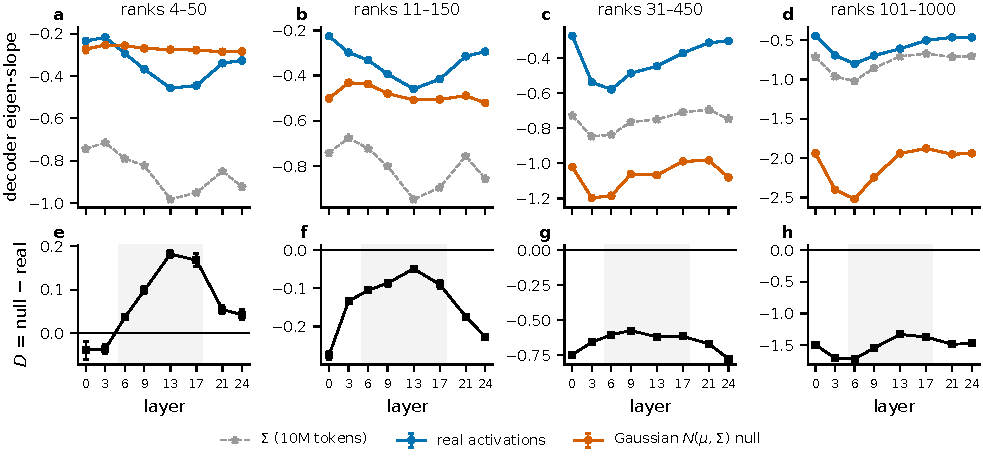
\includegraphics[width=\textwidth]{fig8_null_layers_r2.pdf}
\caption{Real against Gaussian-null SAEs at eight layers of Gemma-2-2B ($k=40$, width 16,384, 8,192 live latents; mean $\pm$ sd over three seeds, dots are seeds, bars mostly smaller than markers; $\Sig$ from the 10M training tokens). (a--d) Decoder eigen-slope. In the top windows the null (orange) barely moves across layers while the real SAE (blue) and $\Sig$ (stars) steepen toward the middle. In the bulk windows the null is 2.0 to 4.4 times steeper than real at every layer, and steeper than $\Sig$. (e--h) $D$, the null's slope minus the real one ($\pm 2$ standard errors; grey band: interior layers of the pre-specified test). In both top windows $D$ peaks at layer 13 and exceeds every end layer by more than 19 standard errors.}
\label{fig:null}
\end{figure}

The Gaussian null is the same TopK SAE trained on samples from $N(\mu,\Sig)$. The scrambled null permutes each coordinate independently across tokens, which keeps every marginal and removes all correlations; its covariance is $\mathrm{diag}(\Sig)$. A random rotation would not serve as a null, because the spectrum is rotation-invariant. The real SAEs leave FVU 0.11--0.29 and the Gaussian-null SAEs 0.52--0.60, so this appendix compares an SAE that finds a sparse code with one that cannot. Real and Gaussian-null SAEs share $\Sig$, so we report raw slopes here. A three-layer set at width 16,384 with a scrambled null gives the same picture, and at layers 3 and 13 its real and Gaussian slopes agree with the eight-layer runs to within 0.003 in every window when both use all live rows.

\subsection{Top-window magnitude}
\label{app:gtop}

In the top windows the Gaussian null's slopes are of the same order as the real ones, and the two differ by layer. Over the eight layers and both top windows, real slopes run from $-0.217$ to $-0.459$ and null slopes from $-0.254$ to $-0.521$; an isotropic cloud of 8,192 points measures about $-0.07$ in ranks 11--150. In ranks 11--150 the null is steeper than real at all eight layers, by 0.05 at layer 13 and up to 0.28 at layer 0. In ranks 4--50 the real SAE is steeper at layers 6 to 24, by up to 0.18 at layer 13, and the null at layers 0 and 3. At layer 13 in ranks 11--150, real minus null $\gamma$ is $-0.09$ at $k=8$ and $+0.18$ at $k=16$, and lies between $-0.05$ and $+0.01$ at every $k$ from 24 to 128. In ranks 4--50 the real $\gamma$ exceeds the null's at every $k$, by 0.07 to 0.48. We have no null at Gemma Scope's own operating point (JumpReLU, $\Lz \approx 76$). Whitening the input does not reduce the decoder to an image of $\Sig$ (Appendix~\ref{app:whiten}).

\subsection{Layer profile}
\label{app:gprofile}

Reading (ii) was fixed before the runs. With $D(L)$ the null's raw slope minus the real one at layer $L$, the profile counts as mid-stack if $D$ is largest at an interior layer (6, 9, 13 or 17) and exceeds $D$ at each end layer (0, 3, 21 and 24) by more than twice their combined seed standard error. Both top windows pass with the maximum at layer 13, where $D$ is $0.182$ in ranks 4--50 and $-0.049$ in ranks 11--150. It exceeds every end layer by at least 0.128 and 0.085. Across the eight layers the null's slope varies by 0.03 in ranks 4--50 and 0.09 in ranks 11--150, against 0.24 and 0.23 for real and 0.27 for $\Sig$. Trained on Gaussian samples, the SAE passes little of $\Sig$'s change across layers to the top of the decoder spectrum, although in the bulk the Gaussian null follows $\Sig$ closely (Pearson $r=0.99$ and 1.00 across layers in ranks 31--450 and 101--1000; post hoc). The equal-power sparse null passes on more of it (a range of 0.13 in both top windows, post hoc).

\subsection{The bulk}
\label{app:gbulk}

At $k=40$ the Gaussian-null SAE is far steeper than the real one in the bulk windows. Its slope is 2.0 to 3.7 times the real slope in ranks 31--450 and 3.1 to 4.4 times in ranks 101--1000. Real is flatter than the null by more than two standard errors at all eight layers in both windows, so the pre-specified bulk reading holds. Real SAEs are flatter than $\Sig$ ($\gamma$ 0.38 to 0.86), and Gaussian-null SAEs are steeper than $\Sig$ itself ($\gamma$ 1.39 to 2.79). In the three-layer set at width 16,384 the scrambled null is 2.1 to 3.4 times steeper than real, except at layer 23 in ranks 101--1000, where its own covariance $\mathrm{diag}(\Sig)$ is nearly flat.

Within the Gaussian $k$ sweep there are two pairs of conditions at similar FVU, chosen after the fact: real $k=8$ against Gaussian $k=64$ (FVU 0.45 and 0.47) and real $k=16$ against Gaussian $k=128$ (0.38 and 0.39), at layer 13 with three seeds each. At both pairs the null is flatter than real in $\gamma$ in both top windows (ranks 11--150: 0.46 against 0.74, and 0.38 against 0.65) and steeper in ranks 101--1000 (2.21 against 1.08, and 1.33 against 0.93). In ranks 31--450 it is steeper at the first pair (1.00 against 0.80) and flatter at the second (0.72 against 0.78).

Along $\Sig$'s bulk axes the real decoder cloud follows a power of $\Sig$ only roughly. The five Gemma Scope layer-12 16k decoder covariances put 0.73--0.77 of their weight on the diagonal of $\Sig$'s eigenbasis, against 0.90--0.98 for an exact $\Sig^{\gamma}$ cloud of the same size (Appendix~\ref{app:matrix}).

\subsection{What the SAE does on Gaussian data}
\label{app:gregime}

A simple account of the steep Gaussian-null bulk is that a TopK SAE on Gaussian data piles near-duplicate latents onto high-variance directions. On 36 local SAEs it does not: the null decoders have fewer near-duplicates than the real ones, and merging near-parallel latents moves no slope by more than 0.003 (Appendix~\ref{app:regime}). The Gaussian null instead follows $\Sig$'s axes more closely. In Pythia-70m its decoder covariance puts 0.95--0.97 of its weight on the diagonal of $\Sig$'s eigenbasis, against 0.80--0.83 for real, and along those axes its exponent in ranks 31--450 is $\gamma=1.21$--3.73 against 0.50--0.76. In the eight-layer Gemma-2-2B runs the diagonal shares are 0.94--0.98 and 0.77--0.84. On Pythia-70m at layer 3 ($k=32$, three widths, three seeds) the Gaussian null is 1.7 to 3.9 times steeper than real in ranks 31--450, and in ranks 11--150 it is 1.5 to 1.6 times steeper.

\subsection{Dependence on $k$}
\label{app:gk}


Reading (i) was that the Gaussian null's $\gamma$ declines as steadily as real's over $k=16$--128: in each window and in both $\gamma$ and raw slope, the null's per-doubling slope must keep real's sign under every leave-one-$k$-out refit and be at least 0.75 of real's (Appendix~\ref{app:ksweep}). The reading is contradicted in ranks 4--50, 11--150 and 101--1000 (Figure~\ref{fig:k}). In ranks 11--150 the real $\gamma$ falls by 0.103 per doubling (seed sd 0.001) and the null's by 0.042 (sd 0.003), a ratio of 0.41; most of the null's change is one step between $k=8$ and 16, where its $\gamma$ falls by 0.36 against 0.09 for real. In ranks 4--50 the null does not decline ($+0.013$ per doubling) while real falls by 0.068. In ranks 31--450 the null declines 4.3 times faster than real and meets the criterion. A resynthesis control that keeps the second moments of Gemma Scope's directions reproduces the small-$k$ drop but only part of the decline above it (Appendix~\ref{app:resynth}).

\subsection{Eight-layer numbers and the three-layer set}
\label{app:65k}

\begin{table}[!htb]
\centering
\caption{Eight layers of Gemma-2-2B at $k=40$, width 16,384: decoder eigen-slope at 8,192 live latents (mean of three seeds), the largest seed sd over the four windows, eval FVU, live latents (range over seeds, of 16,384), and $\Sig$'s slope from the 10M training tokens.}
\label{tab:null8}
\footnotesize
\setlength{\tabcolsep}{4pt}
% generated by paper/figures/make_fig_null_r2.py from results/r2/runs_real.jsonl
\begin{tabular}{r rrrr r r r rr}
\toprule
layer & 4--50 & 11--150 & 31--450 & 101--1000 & max sd & FVU & live & $\Sig$ 11--150 & $\Sig$ 101--1000 \\
\midrule
\multicolumn{10}{l}{\emph{real}} \\
0 & $-0.235$ & $-0.226$ & $-0.273$ & $-0.444$ & 0.009 & 0.114 & 16,384 & $-0.742$ & $-0.713$ \\
3 & $-0.217$ & $-0.298$ & $-0.538$ & $-0.693$ & 0.007 & 0.204 & 16,378--16,383 & $-0.676$ & $-0.961$ \\
6 & $-0.293$ & $-0.332$ & $-0.579$ & $-0.800$ & 0.005 & 0.216 & 16,326--16,358 & $-0.723$ & $-1.019$ \\
9 & $-0.368$ & $-0.393$ & $-0.487$ & $-0.695$ & 0.004 & 0.250 & 16,307--16,345 & $-0.800$ & $-0.855$ \\
13 & $-0.457$ & $-0.459$ & $-0.446$ & $-0.608$ & 0.005 & 0.288 & 16,242--16,272 & $-0.947$ & $-0.705$ \\
17 & $-0.445$ & $-0.416$ & $-0.372$ & $-0.503$ & 0.006 & 0.252 & 16,109--16,172 & $-0.896$ & $-0.671$ \\
21 & $-0.340$ & $-0.315$ & $-0.313$ & $-0.463$ & 0.004 & 0.252 & 16,358--16,365 & $-0.756$ & $-0.713$ \\
24 & $-0.327$ & $-0.294$ & $-0.303$ & $-0.464$ & 0.008 & 0.269 & 16,358--16,370 & $-0.857$ & $-0.703$ \\
\multicolumn{10}{l}{\emph{Gaussian}} \\
0 & $-0.273$ & $-0.501$ & $-1.021$ & $-1.938$ & 0.015 & 0.603 & 16,384 &  &  \\
3 & $-0.254$ & $-0.431$ & $-1.197$ & $-2.401$ & 0.007 & 0.565 & 16,384 &  &  \\
6 & $-0.257$ & $-0.437$ & $-1.184$ & $-2.518$ & 0.004 & 0.530 & 16,384 &  &  \\
9 & $-0.270$ & $-0.479$ & $-1.062$ & $-2.242$ & 0.006 & 0.541 & 16,384 &  &  \\
13 & $-0.275$ & $-0.508$ & $-1.067$ & $-1.939$ & 0.006 & 0.528 & 16,384 &  &  \\
17 & $-0.278$ & $-0.506$ & $-0.989$ & $-1.875$ & 0.011 & 0.557 & 16,384 &  &  \\
21 & $-0.286$ & $-0.489$ & $-0.983$ & $-1.950$ & 0.006 & 0.591 & 16,384 &  &  \\
24 & $-0.284$ & $-0.521$ & $-1.081$ & $-1.938$ & 0.006 & 0.519 & 16,384 &  &  \\
\bottomrule
\end{tabular}

\end{table}

A three-layer set of SAEs, trained with the same recipe at layers 3, 13 and 23, adds the scrambled null and width 65,536 (Tables~\ref{tab:null}--\ref{tab:65k}); it is scored on all live rows. Its width-65,536 SAEs appear undertrained: real $\gamma$ in ranks 11--150 at layer 13 falls from 0.508 at 16k to 0.387 at 65k, a larger change with width than Gemma Scope's SAEs show. No claim in the main text rests on them.

\begin{table}[!htb]
\centering
\caption{Three-layer set: decoder eigen-slope of TopK SAEs at $k=40$, width 16,384, layers 3, 13 and 23, mean of three seeds (largest seed sd 0.013), live rows. $\Sig$ is estimated from the 10M training tokens; the scrambled null's own covariance is $\mathrm{diag}(\Sig)$. FVU and live counts are in Table~\ref{tab:fvu}; width 65,536 is in Table~\ref{tab:65k}. Bold marks the steepest layer for the real SAE in each top window.}
\label{tab:null}
\footnotesize
\setlength{\tabcolsep}{2.6pt}
\begin{tabular}{l rrr rrr rrr rrr}
\toprule
 & \multicolumn{3}{c}{ranks 4--50} & \multicolumn{3}{c}{ranks 11--150} & \multicolumn{3}{c}{ranks 31--450} & \multicolumn{3}{c}{ranks 101--1000} \\
\cmidrule(lr){2-4}\cmidrule(lr){5-7}\cmidrule(lr){8-10}\cmidrule(lr){11-13}
layer & 3 & 13 & 23 & 3 & 13 & 23 & 3 & 13 & 23 & 3 & 13 & 23 \\
\midrule
SAE on real & $-0.224$ & $\mathbf{-0.475}$ & $-0.340$ & $-0.290$ & $\mathbf{-0.481}$ & $-0.292$ & $-0.554$ & $-0.446$ & $-0.280$ & $-0.676$ & $-0.571$ & $-0.389$ \\
SAE on $N(\mu,\Sig)$ & $-0.255$ & $-0.276$ & $-0.286$ & $-0.424$ & $-0.505$ & $-0.507$ & $-1.181$ & $-1.050$ & $-0.972$ & $-2.394$ & $-1.921$ & $-1.841$ \\
SAE on scrambled & $-0.226$ & $-0.391$ & $-0.427$ & $-0.349$ & $-0.649$ & $-0.976$ & $-1.357$ & $-0.954$ & $-0.761$ & $-2.315$ & $-1.241$ & $-0.341$ \\
\midrule
$\Sig$ (10M tokens) & $-0.714$ & $-0.982$ & $-0.807$ & $-0.676$ & $-0.947$ & $-0.749$ & $-0.846$ & $-0.750$ & $-0.697$ & $-0.961$ & $-0.705$ & $-0.679$ \\
\bottomrule
\end{tabular}
\end{table}

\begin{table}[!htb]
\centering
\caption{Regime of the three-layer set ($k=40$): eval FVU (mean of three seeds; seed range $\le 0.003$) and live latents (range over seeds, of 16,384 or 65,536).}
\label{tab:fvu}
\footnotesize
\setlength{\tabcolsep}{2.5pt}
\begin{tabular}{ll rrr}
\toprule
width & condition & layer 3 & layer 13 & layer 23 \\
\midrule
\multirow{3}{*}{16k} & real & 0.204 & 0.288 & 0.287 \\
 & Gaussian & 0.565 & 0.528 & 0.603 \\
 & scrambled & 0.642 & 0.614 & 0.766 \\
\multirow{3}{*}{65k} & real & 0.178 & 0.290 & 0.276 \\
 & Gaussian & 0.559 & 0.526 & 0.594 \\
 & scrambled & 0.636 & 0.610 & 0.747 \\
\midrule
16k live & real & 16.38k & 16.24--16.28k & 16.37--16.38k \\
65k live & real & 65.37--65.41k & 63.97--64.34k & 65.24--65.34k \\
\multicolumn{2}{l}{both nulls, both widths} & \multicolumn{3}{c}{all live except $\le 2$ rows} \\
\bottomrule
\end{tabular}
\end{table}

\begin{table}[!htb]
\centering
\caption{As Table~\ref{tab:null}, at width 65,536 (mean of three seeds). These SAEs appear undertrained (see text) and are reported for completeness only. FVU and live counts are in Table~\ref{tab:fvu}.}
\label{tab:65k}
\footnotesize
\setlength{\tabcolsep}{3pt}
\begin{tabular}{l rrr rrr rrr rrr}
\toprule
 & \multicolumn{3}{c}{ranks 4--50} & \multicolumn{3}{c}{ranks 11--150} & \multicolumn{3}{c}{ranks 31--450} & \multicolumn{3}{c}{ranks 101--1000} \\
\cmidrule(lr){2-4}\cmidrule(lr){5-7}\cmidrule(lr){8-10}\cmidrule(lr){11-13}
layer & 3 & 13 & 23 & 3 & 13 & 23 & 3 & 13 & 23 & 3 & 13 & 23 \\
\midrule
real & $-0.218$ & $-0.286$ & $-0.302$ & $-0.246$ & $-0.366$ & $-0.236$ & $-0.420$ & $-0.367$ & $-0.204$ & $-0.515$ & $-0.413$ & $-0.273$ \\
Gaussian $N(\mu,\Sig)$ & $-0.218$ & $-0.228$ & $-0.280$ & $-0.380$ & $-0.460$ & $-0.497$ & $-0.915$ & $-0.861$ & $-0.875$ & $-1.481$ & $-1.176$ & $-1.167$ \\
scrambled & $-0.211$ & $-0.344$ & $-0.403$ & $-0.331$ & $-0.650$ & $-0.967$ & $-1.053$ & $-0.753$ & $-0.700$ & $-1.517$ & $-0.762$ & $-0.240$ \\
\bottomrule
\end{tabular}
\end{table}

The scrambled null's covariance is $\mathrm{diag}(\Sig)$. Its slopes at layers 3, 13 and 23 are $-0.545$, $-1.166$ and $-0.905$ in ranks 11--150 and $-0.976$, $-0.453$ and $-0.126$ in ranks 101--1000. The flat layer-23 bulk of the scrambled SAE, flatter than real at both widths, follows from the flat $\mathrm{diag}(\Sig)$ there. Its steep layer-23 top window ($-0.976$ at 16k) does not follow from a small denominator, since $\mathrm{diag}(\Sig)$ is steeper there than $\Sig$. The median excess kurtosis of the high-variance coordinates is lowest at layer 23 (0.12, against 0.17 at layer 13 and 0.42 at layer 3), so heavy tails do not explain it either; it remains unexplained.

\section{Whitened-input SAEs}
\label{app:whiten}

\begin{table}[!htb]
\centering
\caption{Whitened-input SAEs at layer 12 (width 16,384, mean of two seeds). Left: decoder eigen-slope in whitened coordinates minus that of an isotropic cloud of the same size (all live rows). Middle: $\gamma$ at 8,192 live latents of the decoder mapped back to the original space, of isotropic whitened-space directions mapped the same way, and of the SAE trained on the same tokens without whitening. Right: eval FVU.}
\label{tab:whiten}
\footnotesize
\setlength{\tabcolsep}{2.5pt}
% generated by paper/figures/make_fig_null_r2.py from results/r2/runs_real.jsonl
\begin{tabular}{r rrrr cccc rr}
\toprule
 & \multicolumn{4}{c}{whitened: slope $-$ isotropic slope} & \multicolumn{4}{c}{$\gamma$: mapped/isotropic mapped/unwhitened} & \multicolumn{2}{c}{FVU} \\
\cmidrule(lr){2-5}\cmidrule(lr){6-9}\cmidrule(lr){10-11}
$k$ & 4--50 & 11--150 & 31--450 & 101--1000 & 4--50 & 11--150 & 31--450 & 101--1000 & whit. & unwh. \\
\midrule
16 & -0.036 & -0.041 & -0.041 & -0.027 & 0.80/0.97/0.52 & 0.78/0.95/0.62 & 0.78/0.96/0.69 & 0.97/1.09/0.89 & 0.615 & 0.363 \\
40 & -0.031 & -0.028 & -0.015 & +0.011 & 0.71/0.97/0.46 & 0.69/0.95/0.50 & 0.66/0.96/0.60 & 0.83/1.08/0.88 & 0.541 & 0.281 \\
128 & +0.007 & +0.015 & +0.026 & +0.023 & 0.64/0.97/0.33 & 0.56/0.95/0.35 & 0.52/0.96/0.51 & 0.70/1.09/0.81 & 0.437 & 0.213 \\
\bottomrule
\end{tabular}

\end{table}

Reading (iii) concerned SAEs trained at layer 12 on activations whitened with $\Sig$ ($k=16$, 40 and 128, two seeds). Their eigen-slopes are within 0.04 of an isotropic cloud's in whitened coordinates. Mapped back through $\Sig^{1/2}$, as described in Appendix~\ref{app:methods}, their $\gamma$ in ranks 11--150 at $k=40$ is 0.69, against 0.95 for mapped isotropic directions and 0.50 for the SAE trained on unwhitened activations. Since the whitened spectrum is close to isotropic, the difference lies in how the directions are placed relative to $\Sig$'s axes. The pre-specified reading, that whitened decoders mapped back are indistinguishable from mapped isotropic directions (within 0.05 in $\gamma$ at all three $k$), is contradicted in all four windows: the mapped $\gamma$ is lower by 0.11 to 0.45, and the gap grows with $k$. Whitened SAEs reconstruct less well than unwhitened ones at every $k$ (FVU 0.44--0.62 against 0.21--0.36).

\section{GPT-2 small}
\label{app:gpt2}

\begin{figure}[!htb]
\centering
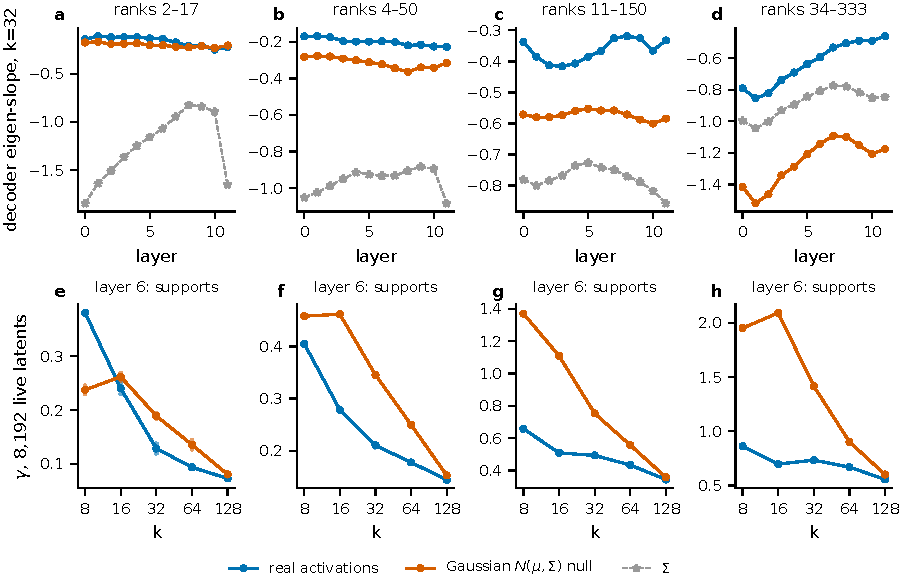
\includegraphics[width=\textwidth]{fig10_gpt2_r2.pdf}
\caption{GPT-2 small, width 16,384, 8,192 live latents, windows scaled to $d=768$ (ranks 4--50 primary). (a--d) Decoder eigen-slope at $k=32$ for real (blue) and Gaussian-null (orange) SAEs at all 12 layers, one seed (two at layer 6, range shown as a bar), and $\Sig$'s slope (stars). Real is flatter than the null in both bulk windows at every layer; in the top windows the real-minus-null difference is largest at the last layers. (e--h) $\gamma$ against $k$ at layer 6, two seeds (dots) and their mean. The null declines with $k$ as steadily as real in every window, unlike Gemma-2-2B at layer 13 (Figure~\ref{fig:k}).}
\label{fig:gpt2}
\end{figure}

The three GPT-2 readings were fixed before the runs. R1, real flatter than the Gaussian null in both bulk windows at every layer by more than two standard errors, holds in every point estimate (Gaussian-to-real slope ratio 1.38--1.81 in ranks 11--150 and 1.78--2.56 in ranks 34--333) but cannot be tested for its margin with one seed per layer, and is therefore partial. R2, a range of the top-window $D$ across layers above $\max(0.05, 2\,\mathrm{se})$, holds in both top windows (0.087 in ranks 2--17, maximum at layer 10; 0.057 in ranks 4--50, maximum at layer 11). The extreme layers have one seed each, so the standard error in that rule was set to zero. $D$ peaks at the last layers, not mid-stack, and in the primary window the null is steeper than real at every layer. R3, that the $k$ test of Appendix~\ref{app:gk} gives the same verdict on GPT-2 as on Gemma-2-2B, fails: on GPT-2 at layer 6 over $k=16$--128 the null declines as steadily as real in all four windows, with per-doubling ratios to real of 1.11, 2.35, 4.42 and 10.2 and leave-one-out minima of 0.86 to 4.6. Real $\gamma$ itself falls by 0.04 to 0.06 per doubling of $k$ in every window. Eval FVU is 0.03--0.18 for real and 0.13--0.44 for Gaussian-null SAEs at $k=32$, and 0.09--0.25 and 0.21--0.61 over $k=8$--128 at layer 6. A sparse null built like Gemma's first one (65,536 sources, 48 active per token) was trained beside the Gaussian null. Its FVU is within 0.002 of the Gaussian null's at all 12 layers, so it is no easier to code, and R3 fails against it too.

\section{The bulk as a matrix law}
\label{app:matrix}

\begin{figure}[!htb]
\centering
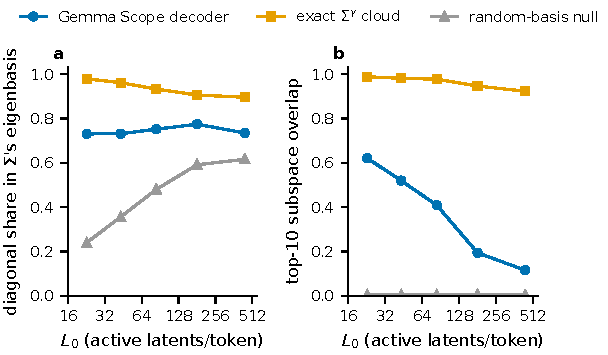
\includegraphics[width=0.85\textwidth]{fig5_matrix_test_1m.pdf}
\caption{Matrix test on the five layer-12 Gemma Scope 16k SAEs ($\Sig$ from 1M tokens; $\Lz$ by release name). (a) Share of the decoder covariance on the diagonal of $\Sig$'s eigenbasis: real decoders 0.73--0.77 at every $\Lz$, between an exact $\Sig^{\gamma}$ cloud of the same size (0.90--0.98) and the decoder's own eigenvalues in a random basis (0.24--0.62). (b) Overlap of the decoder's and $\Sig$'s top-10 eigen-subspaces, falling from 0.62 at $\Lz=22$ to 0.12 at $\Lz=445$, against 0.92--0.99 for the exact cloud.}
\label{fig:matrix}
\end{figure}

We rotate the decoder covariance into $\Sig$'s eigenbasis, regress its log diagonal on $\log\lambda^{\Sig}$, and compare with two synthetic clouds of 16,384 unit rows (Figure~\ref{fig:matrix}). Over ranks 101--1000 the regression has $R^2=0.955$--0.989 at every $\Lz$ and gives exponents from 0.81 ($\Lz=22$ by release name) to 0.37 ($\Lz=445$). In ranks 11--150 it holds only at low $\Lz$ ($R^2 = 0.94$--0.98 up to $\Lz=82$, 0.73 at 176 and 0.01 at 445); at high $\Lz$ the top of the decoder spectrum stops following $\Sig$'s leading directions. Placing each decoder's own eigenvalues in a random basis gives $R^2 \le 0.003$ over ranks 101--1000 and $\le 0.012$ in any window. The same test on local Gaussian-null decoders is in Appendix~\ref{app:gregime}.

\section{Resynthesis}
\label{app:resynth}

\begin{figure}[!htb]
\centering
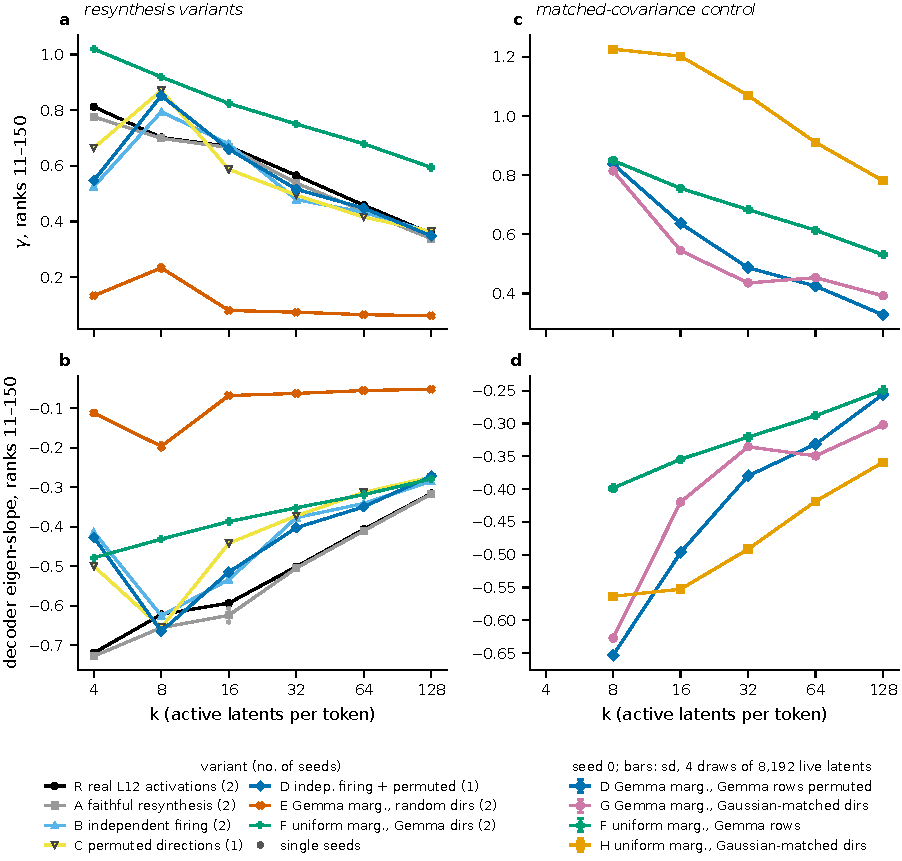
\includegraphics[width=\textwidth]{fig6_resynthesis.pdf}
\caption{Resynthesis at layer 12, ranks 11--150. Left: variants R (real activations), A (faithful resynthesis from codes), B (independent firing), C (permuted decoder rows), D (B and C), E (random directions), F (uniform firing on Gemma Scope's rows); $\gamma$ (a) and raw slope (b). Right: the matched-covariance control at a fixed 8,192 live latents for one draw and one seed (bars: sd over four draws of live latents); Figure~\ref{fig:resynth2} has all three draws and both seeds.}
\label{fig:resynth}
\end{figure}

We encoded layer-12 activations with the Gemma Scope 65k SAE ($\Lz=72$) and resynthesised training data from its codes, firing each latent independently with its empirical frequency and value distribution, either on Gemma Scope's decoder rows re-paired at random (variant D) or on directions drawn from a Gaussian with those rows' mean and covariance (variant G). Each variant of Figure~\ref{fig:resynth} breaks one ingredient of the resynthesis. The faithful resynthesis A keeps the real $\gamma(k)$ (per-doubling $-0.095$ over $k=8$--128, against $-0.090$ for real activations). Variants that keep Gemma Scope's directions or their pairing with frequencies keep the decline ($-0.111$ to $-0.122$; C and D one seed). Random directions (E) give $-0.036$, from a curve at the isotropic floor. Uniform firing on Gemma Scope's rows (F) gives $-0.080$ in $\gamma$ but only $-0.037$ in raw slope; F's covariance is the dictionary's own, whose slope ($-0.469$) is the decoder slope of the source SAE, so F is close to circular. The control variant H (uniform firing on Gaussian-matched directions) starts above $\gamma=1$ and recovers little (FVU 0.67 at $k=8$, against 0.50 for F).

\begin{figure}[!htb]
\centering
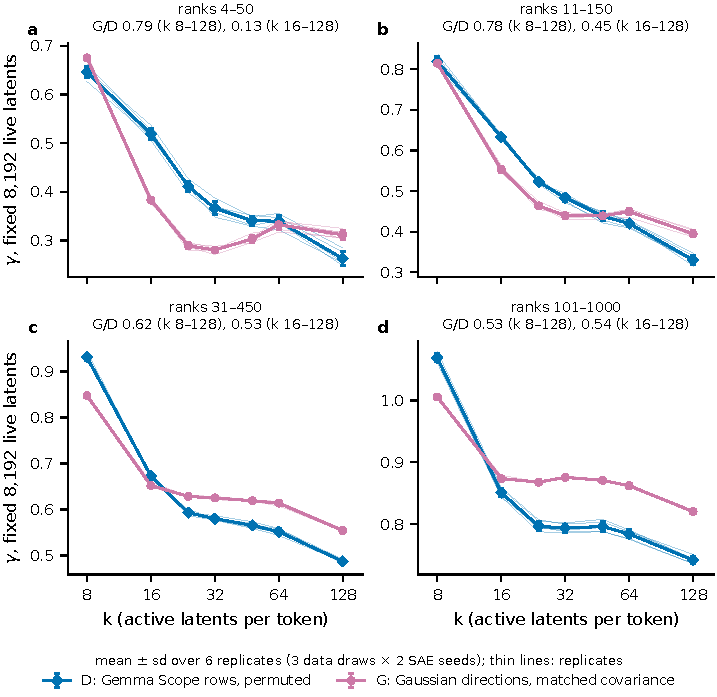
\includegraphics[width=0.9\textwidth]{fig7_resynth_r2.pdf}
\caption{Control G against D at layer 12, width 16,384, in the four rank windows: $\gamma$ at a fixed 8,192 live latents, mean $\pm$ sd over six replicates (three draws of directions and codes, two SAE seeds each); thin lines are single replicates. G follows D's drop between $k=8$ and 16 and then flattens, most clearly in ranks 4--50, while D keeps falling. Panel titles give G's retention of D's per-doubling slope over $k=8$--128 (pre-specified) and $k=16$--128 (post hoc).}
\label{fig:resynth2}
\end{figure}

\begin{table}[!htb]
\centering
\caption{Control G against D: per-doubling slope of $\gamma$ in $k$ for each variant (mean $\pm$ sd over six replicates) and G's retention of D's slope, in $\gamma$ and raw slope, with paired two-level bootstrap 95\% intervals (draws, then seeds within draws; 20,000 resamples). The verdict uses the fixed-$n$ columns: keeps at $\ge 0.75$ in both units, removes below 0.5 in both. Full-live-count retention is reported only.}
\label{tab:resynth2}
\small
% generated by paper/figures/make_fig_resynth_r2.py from results/r2/resynth_analysis.json
\begin{tabular}{l rr ll rr l}
\toprule
 & \multicolumn{4}{c}{fixed 8,192 live latents} & \multicolumn{2}{c}{full live count} & \\
\cmidrule(lr){2-5}\cmidrule(lr){6-7}
ranks & $s_D$ ($\gamma$) & $s_G$ ($\gamma$) & G/D $\gamma$ [95\%] & G/D raw [95\%] & G/D $\gamma$ & G/D raw & verdict \\
\midrule
\multicolumn{8}{l}{\emph{$k=8$--128 (pre-registered)}} \\
4--50 & $-0.094 \pm 0.002$ & $-0.074 \pm 0.002$ & 0.79 [0.777, 0.810] & 0.79 [0.776, 0.799] & 0.80 & 0.80 & keeps \\
11--150 & $-0.118 \pm 0.004$ & $-0.092 \pm 0.001$ & 0.78 [0.760, 0.798] & 0.76 [0.748, 0.779] & 0.79 & 0.78 & keeps \\
31--450 & $-0.098 \pm 0.001$ & $-0.060 \pm 0.001$ & 0.62 [0.605, 0.624] & 0.62 [0.608, 0.628] & 0.61 & 0.62 & partial \\
101--1000 & $-0.069 \pm 0.001$ & $-0.036 \pm 0.001$ & 0.53 [0.520, 0.533] & 0.54 [0.531, 0.553] & 0.52 & 0.54 & partial \\
\multicolumn{8}{l}{\emph{$k=16$--128 (post hoc)}} \\
4--50 & $-0.076 \pm 0.002$ & $-0.010 \pm 0.003$ & 0.13 [0.104, 0.164] & 0.13 [0.104, 0.161] & 0.11 & 0.11 & removes \\
11--150 & $-0.093 \pm 0.004$ & $-0.042 \pm 0.002$ & 0.45 [0.432, 0.457] & 0.44 [0.423, 0.449] & 0.46 & 0.45 & removes \\
31--450 & $-0.054 \pm 0.001$ & $-0.029 \pm 0.001$ & 0.53 [0.513, 0.542] & 0.53 [0.517, 0.544] & 0.52 & 0.52 & partial \\
101--1000 & $-0.030 \pm 0.001$ & $-0.016 \pm 0.001$ & 0.54 [0.518, 0.557] & 0.55 [0.532, 0.575] & 0.52 & 0.53 & partial \\
\bottomrule
\end{tabular}

\end{table}

G is sparsely codable and its FVU tracks D's (0.398 against 0.417 at $k=8$, 0.191 against 0.175 at $k=128$). We trained 84 SAEs (three draws of directions and codes, two seeds, seven $k$) and fixed a rule beforehand: G \emph{keeps} D's decline if it retains at least 0.75 of D's per-doubling slope over $k=8$--128 in both $\gamma$ and raw slope, and \emph{removes} it below 0.5 in both, applied to the mean slope over draws, with the window rule. In ranks 11--150 G retains 0.78 of D's decline in $\gamma$ (bootstrap interval $[0.760, 0.798]$) and 0.76 in raw slope ($[0.748, 0.779]$), so the raw interval reaches just below the threshold; it retains 0.79 in ranks 4--50, 0.62 in ranks 31--450 and 0.53 in ranks 101--1000, so the pre-specified reading is mixed. G reproduces and exceeds D's step between $k=8$ and 16 ($\gamma$ falls by 0.26 for G and 0.19 for D in ranks 11--150) and then flattens, the shape of the Gaussian null's curve in Figure~\ref{fig:k}. Over $k=16$--128, a range chosen post hoc, G retains 0.45 in ranks 11--150 (interval $[0.43, 0.46]$), 0.13 in ranks 4--50 and 0.53--0.54 in the bulk, and leaving out one $k$ at a time over $k=8$--128 gives 0.45 to 0.88. Second moments of the dictionary, with independent sparse codes, therefore account for the small-$k$ drop and not for much of the decline above it. The equal-power sparse null, whose atoms are random directions shaped by $\Sig$, stays within 0.08 of real's $\gamma$ at every $k \ge 24$ while declining 1.44 times as fast (Appendix~\ref{app:primary}), so matching the level of that curve does not need Gemma Scope's directions.

Each draw of directions and codes is independent, and at a given draw D and G share the same code draws, so the comparison is paired. The firing frequencies and 64-quantile value distributions come from Gemma Scope's codes on the first 4M real layer-12 training tokens. Each synthetic dataset has 12M tokens, of which the last 0.5M are held out, and each SAE makes three passes over the other 11.5M. $\gamma$ for each SAE uses the $\Sig$ of its own synthetic dataset, estimated from its 12M tokens. The per-draw retention in ranks 11--150 runs from 0.76 to 0.80 in $\gamma$ and from 0.75 to 0.78 in raw slope, and every draw gives the same verdict as the mean in every window. Scoring at the full live count changes no retention by more than 0.02. In ranks 11--150 G's mean $\gamma$ at $k=8$, 16, 24, 32, 48, 64 and 128 is 0.815, 0.553, 0.464, 0.440, 0.439, 0.449 and 0.395, and D's is 0.820, 0.633, 0.523, 0.484, 0.438, 0.420 and 0.330 (sd over replicates at most 0.011). $\Sig$'s slope in ranks 11--150 is $-0.77$ to $-0.79$ for every resynthesised dataset. At the first draw and seed, D reproduces the single-draw run of Figure~\ref{fig:resynth} exactly and G within 0.007 in $\gamma$.

\section{Layer-13 $k$ sweep: details}
\label{app:ksweep}

The test of Appendix~\ref{app:gk} fits, per seed, the slope of $\gamma$ (and of the raw decoder slope) on $\log_2 k$ over $k=16$, 24, 32, 48, 64 and 128. The null's per-doubling slope supports the reading if it has real's sign by more than two standard errors and under every leave-one-$k$-out refit, and is at least 0.75 of real's. It contradicts the reading if it is flat or changes sign under a refit, or if it is below 0.5 of real's by more than two standard errors. In ranks 11--150, without $k=128$ the Gaussian null's slope is 0.009, and after its step between $k=8$ and 16 its $\gamma$ rises to 0.56 at $k=32$ and falls again. In ranks 101--1000 the Gaussian null is not monotone (1.76 at $k=16$, 2.82 at 32, 1.33 at 128). In ranks 31--450 it declines by 0.327 per doubling against 0.077 for real. Including the step, over $k=8$--128, it falls by 0.089 per doubling in ranks 11--150 against 0.104 for real.

\section{Near-duplicates and axes in local SAEs}
\label{app:regime}

We kept only the decoder covariances of the eight-layer runs, so the near-duplicate account of Appendix~\ref{app:gregime} was tested on 36 local SAEs, in which the null decoders have fewer near-duplicates than the real ones. They are Pythia-70m layer 3 at three widths, three seeds and three conditions, and Gemma-2-2B width-4096 $k=40$ SAEs (real and Gaussian at layer 12; Gaussian at seven more layers). In Pythia, the 99th percentile of each latent's maximum cosine to another latent is 0.29--0.33 for the Gaussian null against 0.42--0.46 for real. The share of latents with a neighbour above cosine 0.5 is 0.07--0.16\% against 0.17--0.43\%. Merging near-parallel latents at any threshold removes at most 0.39\% of rows. At Gemma layer 12 the shares of the decoder covariance on the diagonal of $\Sig$'s eigenbasis are 0.87 (Gaussian) against 0.82 (real), with random-basis benchmarks of 0.21 and 0.34. The scrambled null puts less weight than real on $\Sig$'s diagonal (0.67--0.73 in Pythia) and 0.93--0.99 on the diagonal of its own covariance $\mathrm{diag}(\Sig)$. Within this local set the Gaussian-null decoder is close to a $\Sig^{\gamma}$ cloud with large $\gamma$, and the real decoder departs further from $\Sig$'s axes.

The Pythia slopes of Appendix~\ref{app:gregime} are on all live rows. Real and Gaussian-null SAEs agree in ranks 4--50 ($-0.31$ to $-0.32$ against $-0.27$ to $-0.37$); in ranks 11--150 the null gives $-0.60$ to $-0.62$ against $-0.38$ to $-0.41$. FVU is 0.11--0.14 for real and 0.22--0.24 for Gaussian-null SAEs.

\section{Cluster structure across layers}
\label{app:cluster}

If the mid-stack top window reflects structure beyond $\Sig$, the decoder cloud should cluster more than a covariance-matched cloud does. We clustered the decoder directions of the 16k Gemma Scope SAE nearest $\Lz=70$ at each of the 26 layers (spherical $k$-means, 1,024 and 256 clusters), did the same for a unit-normalised Gaussian cloud with the decoder cloud's own covariance, and count only the excess over it: the excess between-cluster share of variance and the excess cosine to the cluster centre. With 1,024 clusters the excess correlates with the top-window slope at Spearman $\rho=-0.874$ to $-0.910$ (phase-surrogate $p<10^{-4}$; circular shifts give $p=0.038$, the floor for 26 layers). The excess statistics also correlate with $\Sig$'s slope ($\rho=-0.80$ to $-0.82$). Controlling for $\Sig$'s slope leaves partial $\rho=-0.63$ to $-0.78$ (phase $p=0.006$--0.030). Controlling as well for the matched cloud's own clustering leaves $-0.40$ to $-0.58$; the excess cosine stays significant (phase $p=0.009$ and 0.043) and the excess share does not ($p=0.064$ and 0.082). With 256 clusters, $\rho=-0.79$ to $-0.90$, but one cell (excess share, ranks 4--50) has shift $p=0.31$. Two of the four cells fall below the pre-stated survival rule after controlling for $\Sig$ (partial $\rho=-0.64$, $p=0.069$; $-0.57$, $p=0.052$). In the bulk windows $|\rho| \le 0.14$ with 1,024 clusters, and $\rho=-0.42$ and $-0.45$ (not significant) for the excess share with 256. The analysis uses Gemma Scope decoders at one $\Lz$, holds only in the two top windows, which share most of their ranks, does not meet the window rule, and has not been run on our real and null SAEs.

\clearpage

\section{Explanations that fail, and planted data}
\label{app:fail}

\textbf{Feature splitting.} If near-parallel latents acted as large spikes, removing them would flatten the spectrum. We greedily merged latents with cosine above 0.5 in 22 layer-12 Gemma Scope SAEs. This removed up to 34.5\% of latents (131k, $\Lz=12$) and changed the ranks 11--150 slope by at most 0.010.

\textbf{Massive activations.} One residual dimension carries rare, very large values. Training our layer-13 16k $k=40$ SAEs (three seeds) without the tokens carrying its top 0.1\% or 1\% of values changed $\gamma$ by at most 0.0052 (ranks 4--50) and at most 0.0017 in the other windows. This test was run at one layer only.

\textbf{Latent-frequency allocation.} \citet{michaud2025manifolds} derive an exponent for the number of latents allocated per feature. If decoder eigenvalues scaled with the number of latents per feature, which is our assumption and not theirs, the eigen-slope would inherit that exponent and would move with $\Lz$ through the frequency distribution. Across 22 layer-12 SAEs the rank-frequency exponent of latent firing (ranks 10 to the last live latent) runs from $-0.59$ to $-0.91$ for $\Lz < 270$ and steepens to $-0.93$ to $-1.01$ at $\Lz \ge 270$, where the decoder slope is flattest. For the 18 SAEs with $\Lz < 270$ the pooled rank correlation with $\Lz$ is 0.13, and within width the trend per doubling of $\Lz$ is $-0.004$ (16k), $+0.009$ (32k), $-0.012$ (65k) and $-0.043$ (131k). Over all 22 SAEs the exponent's rank correlation with the decoder slope in ranks 11--150 is $-0.37$ ($p=0.09$), and 0.14 ($p=0.59$) for $\Lz < 270$. Latent frequencies are not feature frequencies, so this leaves the allocation account underdetermined.

\textbf{Planted features.} Synthetic activations built as sparse sums of planted features at $d=2{,}304$, with $\Sig$'s slope matched to Gemma's in every window, did not reproduce Gemma's $\gamma(k)$ in ranks 11--150. The best root-mean-square distance to Gemma's curve was 0.27 without clusters and 0.24 with planted clusters of 16 features at cosine 0.6 to a centre, against a pre-specified pass test of RMS below 0.15 and a per-doubling slope within 0.04 of Gemma's. Over $k=4$--128 every planted curve was nearly flat ($-0.009$ to $+0.018$ per doubling for seven generators, against $-0.095$ for Gemma over the same range). Five of the seven generators ran one seed and two ran two. The generator with 4,608 features has a jagged curve and gives $-0.074$ over $k=8$--128. A point-feature generator whose $\Sig$ was not slope-matched (it has a plateau over its top eigenvalues) came within RMS 0.14 of Gemma's curve on one seed, but its $\gamma$ falls by only 0.041 per doubling over $k=4$--128 and fails the slope part of that test.

\section{Activation spectra under other protocols}
\label{app:li}

\begin{table}[!htb]
\centering
\caption{Layer 12, 1M tokens: eigen-slope of the activation spectrum under five preprocessing choices, against the decoder of \citeauthor{li2025geometry}'s SAE (65k, $\Lz=72$ by release name, 75.9 measured on 1M tokens).}
\label{tab:li}
\small
\begin{tabular}{l rrrr}
\toprule
 & ranks 1--100 & 11--150 & 31--450 & 101--1000 \\
\midrule
decoder cloud (centred) & $-0.462$ & $-0.468$ & $-0.418$ & $-0.503$ \\
activations, raw, centred ($\Sig$) & $-0.923$ & $-0.883$ & $-0.732$ & $-0.717$ \\
activations, raw, uncentred & $-1.031$ & $-0.902$ & $-0.739$ & $-0.718$ \\
activations, unit-norm tokens, centred & $-0.880$ & $-0.864$ & $-0.748$ & $-0.731$ \\
activations, unit-norm tokens, uncentred & $-1.012$ & $-0.881$ & $-0.753$ & $-0.732$ \\
activations, per-dimension standardised & $-0.446$ & $-0.489$ & $-0.535$ & $-0.600$ \\
\bottomrule
\end{tabular}
\end{table}

Li et al.'s exponent for the decoder is fitted over ranks 11--150, and their activation-to-feature comparison uses the 100 largest eigenvalues. Their protocol for the activations is not given, so we varied it at layer 12 against their SAE. Table~\ref{tab:li} gives the layer-12 grid; unit-normalised tokens, uncentred activations and the SAE's own codes give $-0.88$ to $-1.03$ in ranks 1--100. With fewer tokens the raw spectrum flattens (ranks 1--100: $-0.63$ at 256 tokens, $-0.78$ at 1,024, $-0.91$ at 16,384) but stays steeper than the decoder. Reading ``activations'' as the SAE's codes gives $-0.987$ (ranks 1--100).

At all 26 layers, on the 1M-token covariance, we compared the activation spectrum with two decoders: Li et al.'s 65k SAE at each layer, and the 16k SAE whose $\Lz$ is nearest 40. Under the raw centred and raw uncentred covariance the activation spectrum is steeper than both decoders at 26 of 26 layers in every window ($\gamma$ 0.26--0.60 in ranks 1--100 and 11--150). Under the correlation matrix, Li et al.'s ordering holds in ranks 1--100 at layers 11--14 against their SAEs (4 of 26; 2 of 26 in ranks 11--150) and at layers 10--18 against the 16k SAEs (9 of 26; 8 of 26 in ranks 11--150), with $\gamma$ up to 1.15 and 1.28. The correlation-matrix spectrum is the most sensitive to sample size: at layer 12 it is $-0.544$ on 32,736 tokens and $-0.446$ on 1M. We could not test other models, hooks or text distributions.

\end{document}
